%%% The main file. It contains definitions of basic parameters and includes all other parts.

%% Settings for single-side (simplex) printing
% Margins: left 40mm, right 25mm, top and bottom 25mm
% (but beware, LaTeX adds 1in implicitly)
%\documentclass[12pt,a4paper]{report}
%\setlength\textwidth{145mm}
%\setlength\textheight{247mm}
%\setlength\oddsidemargin{15mm}
%\setlength\evensidemargin{15mm}
%\setlength\topmargin{0mm}
%\setlength\headsep{0mm}
%\setlength\headheight{0mm}
% \openright makes the following text appear on a right-hand page
%\let\openright=\clearpage

%% Settings for two-sided (duplex) printing
\documentclass[12pt,a4paper,twoside]{report}
% \setlength\textwidth{145mm}
% \setlength\textheight{247mm}
% \setlength\oddsidemargin{14.2mm}
% \setlength\evensidemargin{0mm}
% \setlength\topmargin{0mm}
% \setlength\headsep{0mm}
% \setlength\headheight{0mm}
\let\openright=\cleardoublepage

%% Generate PDF/A-2u
\usepackage[a-2u]{pdfx}
\usepackage{algorithm}
\usepackage{comment}
\usepackage{algpseudocode}

%% Character encoding: usually latin2, cp1250 or utf8:
\usepackage[utf8]{inputenc}

% Let's use a decent modern font
\usepackage[T1]{fontenc}
\usepackage[mono=false]{libertine}
%other choices -- URW schoolbook: 
%\usepackage{fouriernc}
% or URW palladio
%\usepackage[sc]{mathpazo}
%\linespread{1.05}

%% Further useful packages (included in most LaTeX distributions)
\usepackage{amsmath}        % extensions for typesetting of math
\usepackage{amsfonts}       % math fonts
\usepackage{amsthm}         % theorems, definitions, etc.
\usepackage{bbding}         % various symbols (squares, asterisks, scissors, ...)
\usepackage{bm}             % boldface symbols (\bm)
\usepackage{graphicx}       % embedding of pictures
\usepackage{fancyvrb}       % improved verbatim environment
\usepackage[style=numeric,natbib=true,backend=bibtex,style=alphabetic]{biblatex}
\addbibresource{bibliography.bib}
\defbibheading{Bibliography}{}

\usepackage[nottoc]{tocbibind} % makes sure that bibliography and the lists
			    % of figures/tables are included in the table
			    % of contents
\usepackage{dcolumn}        % improved alignment of table columns
\usepackage{booktabs}       % improved horizontal lines in tables
\usepackage{paralist}       % improved enumerate and itemize
%\usepackage[usenames]{xcolor}  % typesetting in color
\usepackage[textsize=tiny, color=yellow!30]{todonotes}
\usepackage{longtable}
\usepackage{subcaption}

\newcommand{\xxx}[1]{\textcolor{red}{#1}}

%%% Basic information on the thesis

% Thesis title in English (exactly as in the formal assignment)
\def\ThesisTitle{OCR for tabular data}

% Author of the thesis
\def\ThesisAuthor{Lucia Tódová}

% Year when the thesis is submitted
\def\YearSubmitted{2019}

% Name of the department or institute, where the work was officially assigned
% (according to the Organizational Structure of MFF UK in English,
% or a full name of a department outside MFF)
\def\Department{Department of Software Engineering}

% Is it a department (katedra), or an institute (ústav)?
\def\DeptType{Department}

% Thesis supervisor: name, surname and titles
\def\Supervisor{Mgr. Miroslav Kratochvíl}

% Supervisor's department (again according to Organizational structure of MFF)
\def\SupervisorsDepartment{Department of Software Engineering}

% Study programme and specialization
\def\StudyProgramme{Computer Science}
\def\StudyBranch{Programming and Software Systems}

% An optional dedication: you can thank whomever you wish (your supervisor,
% consultant, a person who lent the software, etc.)
\def\Dedication{%
Dedication.
}

% Abstract (recommended length around 80-200 words; this is not a copy of your thesis assignment!)
\def\Abstract{%
Abstract.
}

% 3 to 5 keywords (recommended), each enclosed in curly braces
\def\Keywords{%
{key} {words}
}

%% The hyperref package for clickable links in PDF and also for storing
%% metadata to PDF (including the table of contents).
%% Most settings are pre-set by the pdfx package.
\hypersetup{unicode}
\hypersetup{breaklinks=true}

% Definitions of macros (see description inside)
%%% This file contains definitions of various useful macros and environments %%%
%%% Please add more macros here instead of cluttering other files with them. %%%

%%% Minor tweaks of style

% These macros employ a little dirty trick to convince LaTeX to typeset
% chapter headings sanely, without lots of empty space above them.
% Feel free to ignore.
\makeatletter
\def\@makechapterhead#1{
  {\parindent \z@ \raggedright \normalfont
   \Huge\bfseries \thechapter. #1
   \par\nobreak
   \vskip 20\p@
}}
\def\@makeschapterhead#1{
  {\parindent \z@ \raggedright \normalfont
   \Huge\bfseries #1
   \par\nobreak
   \vskip 20\p@
}}
\makeatother

% This macro defines a chapter, which is not numbered, but is included
% in the table of contents.
\def\chapwithtoc#1{
\chapter*{#1}
\addcontentsline{toc}{chapter}{#1}
}

% Draw black "slugs" whenever a line overflows, so that we can spot it easily.
%\overfullrule=1mm
% TODO: comment this out for typesetting the final version. Most black slugs can be removed by correctly\-breaking\-the\-long\-words\-using\-backslashed\-hyphen
%\emergencystretch=1ex %this prevents a lot of slugs.

%%% Macros for definitions, theorems, claims, examples, ... (requires amsthm package)

\theoremstyle{plain}
\newtheorem{thm}{Theorem}
\newtheorem{lemma}[thm]{Lemma}
\newtheorem{claim}[thm]{Claim}

\theoremstyle{plain}
\newtheorem{defn}{Definition}

\theoremstyle{remark}
\newtheorem*{cor}{Corollary}
\newtheorem*{rem}{Remark}
\newtheorem*{example}{Example}

%%% An environment for proofs

%%% FIXME %%% \newenvironment{proof}{
%%% FIXME %%%   \par\medskip\noindent
%%% FIXME %%%   \textit{Proof}.
%%% FIXME %%% }{
%%% FIXME %%% \newline
%%% FIXME %%% \rightline{$\square$}  % or \SquareCastShadowBottomRight from bbding package
%%% FIXME %%% }

%%% An environment for typesetting of program code and input/output
%%% of programs. (Requires the fancyvrb package -- fancy verbatim.)

\DefineVerbatimEnvironment{code}{Verbatim}{fontsize=\small, frame=single}

%%% The field of all real and natural numbers
\newcommand{\R}{\mathbb{R}}
\newcommand{\N}{\mathbb{N}}

%%% Useful operators for statistics and probability
\DeclareMathOperator{\pr}{\textsf{P}}
\DeclareMathOperator{\E}{\textsf{E}\,}
\DeclareMathOperator{\var}{\textrm{var}}
\DeclareMathOperator{\sd}{\textrm{sd}}

%%% Transposition of a vector/matrix
\newcommand{\T}[1]{#1^\top}

%%% Various math goodies
\newcommand{\goto}{\rightarrow}
\newcommand{\gotop}{\stackrel{P}{\longrightarrow}}
\newcommand{\maon}[1]{o(n^{#1})}
\newcommand{\abs}[1]{\left|{#1}\right|}
\newcommand{\dint}{\int_0^\tau\!\!\int_0^\tau}
\newcommand{\isqr}[1]{\frac{1}{\sqrt{#1}}}

%%% Various table goodies
\newcommand{\pulrad}[1]{\raisebox{1.5ex}[0pt]{#1}}
\newcommand{\mc}[1]{\multicolumn{1}{c}{#1}}


% Title page and various mandatory informational pages
\begin{document}
%%% Title page of the thesis and other mandatory pages

%%% Title page of the thesis

\pagestyle{empty}
\hypersetup{pageanchor=false}
\begin{center}

\centerline{\mbox{
\includegraphics[width=166mm]{../img/logo-en.pdf}}}

\vspace{-8mm}
\vfill

{\bf\Large BACHELOR THESIS}

\vfill

{\LARGE\ThesisAuthor}

\vspace{15mm}

{\LARGE\bfseries\ThesisTitle}

\vfill

\Department

\vfill

\begin{tabular}{rl}

Supervisor of the bachelor thesis: & \Supervisor \\
\noalign{\vspace{2mm}}
Study programme: & \StudyProgramme \\
\noalign{\vspace{2mm}}
Study branch: & \StudyBranch \\
\end{tabular}

\vfill

% Zde doplňte rok
Prague \YearSubmitted

\end{center}

\newpage

%%% Here should be a bound sheet included -- a signed copy of the "bachelor
%%% thesis assignment". This assignment is NOT a part of the electronic
%%% version of the thesis. DO NOT SCAN.

%%% A page with a solemn declaration to the bachelor thesis

\openright
\hypersetup{pageanchor=true}
\pagestyle{plain}
\pagenumbering{roman}
\vglue 0pt plus 1fill

\noindent
I declare that I carried out this bachelor thesis independently, and only with the cited
sources, literature and other professional sources.

\medskip\noindent
I understand that my work relates to the rights and obligations under the Act No.~121/2000 Sb.,
the Copyright Act, as amended, in particular the fact that the Charles
University has the right to conclude a license agreement on the use of this
work as a school work pursuant to Section 60 subsection 1 of the Copyright Act.

\vspace{10mm}

\hbox{\hbox to 0.5\hsize{%
In ........ date ............	% FIXME!
\hss}\hbox to 0.5\hsize{%
signature of the author
\hss}}

\vspace{20mm}
\newpage

%%% Dedication

\openright

\noindent
\Dedication

\newpage

%%% Mandatory information page of the thesis

\openright

\vbox to 0.5\vsize{
\setlength\parindent{0mm}
\setlength\parskip{5mm}

Title:
\ThesisTitle

Author:
\ThesisAuthor

\DeptType:
\Department

Supervisor:
\Supervisor, \SupervisorsDepartment

Abstract:
\Abstract

Keywords:
\Keywords

\vss}

\newpage

\openright
\pagestyle{plain}
\pagenumbering{arabic}
\setcounter{page}{1}


%%% A page with automatically generated table of contents of the bachelor thesis

\tableofcontents

%%% Each chapter is kept in a separate file
\chapter*{Introduction}
\addcontentsline{toc}{chapter}{Introduction}

Recently, digitalization of documents has become an important part of information systems and related workflows. By digitalization, documents from governmental, administrative, educational and publishing workflows are being processed to a more accessible, searchable and manageable form.

To convert the printed text documents back into digital text form, digitalization tools employ \emph{optical character recognition} (OCR). OCR engines are used to recognize individual text elements of a scanned document and output them in a more suitable format, e.g.~as rich text or a searchable PDF file.

Specialized OCR algorithms exist to handle various specific input document layouts where general OCR would produce sub-optimal or unusuable results; e.g. for tickets, passports, car plates or postal envelopes. Tabular documents form a wide, useful category of structured input --- table recognition algorithms must be able to process various features found in the tables, including inconsistent border formatting, different alignment, spanning cells, or misaligned columns and rows. Currently, the available table-recognition software is, in most cases, derived from text-oriented OCR algorithms and recognizes only limited amount of all possible table features.

The main goal of this thesis is to explore the existing OCR techniques and software, and create a new table recognition OCR software that can provide better results than the currently available tools. The resulting software uses an external OCR engine and image-processing libraries to preprocess the input images and extract simple text elements, which are then heuristically combined into words, lines, table columns and whole tables. Finally, it produces an easily readable JSON-formatted output that describes the layouts of tabular and textual elements in the processed document. The generalized JSON output may be eventually converted to other, more specific formats.

\subsection*{Related work}

There exist several softwares that focus on table recognition. For example, Tabula~\cite{Tabula} is an under development open-source project focusing on the extraction of tables from PDF files. This software uses the help of the OpenCV library~\cite{OpenCV} and often results in errors when presented with scanned documents, multi-line rows and complex tables. Another examples are OCRSpace~\cite{OCRSpace} and OpenCV~\cite{OpenCV}. Although the focus of these engines is mainly character recognition, they also provide table recognition of specific layouts (e.g. receipts, tickets). Other approaches to table recognition were presented by~\citet{pdf2table},~\citet{TRecs} and~\citet{MediumTable}. Even though they proposed new techniques, they are now either outdated or do not provide results of sufficient quality. Satisfactory results are provided by commercial softwares like ABBYY FineReader~\cite{ABBYYdpi}.

Table recognition is also implemented as a feature of the Tesseract library~\cite{tableDetHeterogeneous}. We discuss it in detail later in this thesis (\cref{tableFind}).

\paragraph{Layout of this thesis} This thesis is structured as follows: In Chapter 1, we review the obstacles that complicate character recognition and show existing solutions for some of them; after that we describe several techniques and heuristics for text recognition. In Chapter 2, we describe the implementation of existing table recognition algorithms. Chapter 3 details the implementation of our software, including the heuristic used for table detection and recognition. Performance measurements, results and summary of the improvements are presented in Chapter 4. After the last chapter, we conclude with a brief overview of possible future work.

\chapter{Text Recognition Algorithms}

The root of any complex OCR software is text recognition.\todo{tady urcite chces nejakej pokec o tom co v ty kapitole vlastne bude: Prolezeme hlavni problemy se kterejma se text recognition potyka, pak si ukazeme hlavni metodu implementace ktera postupuje od jednoduchyho predzpracovani obrazku, pres hledani a rozpoznavani glyf az ke skupinkovani glyf do slov a textu.}
Although this is easily done in printed documents\todo{Is this valid for documents printed with skewed red comic-sans bold, on a green background with purple cats?}, there can be a lot of factors that complicate this process.
\citet{preprocessAll} describe the following major difficulties that complicate the text recognition process:

\begin{description}
\item[Font face variability] Nowadays, a multitude of different fonts and styles is used in the documents\todo{vklidu se opri do toho ze lidi si kamkoliv strcej bold nebo italics a nezajima je citelnost :D }. To hold the information about each and every one would be unsustainable for any OCR software \todo{why not?}. Therefore, it needs to make assumptions and use heuristics to match its \xxx{vision}\todo{expectation?} of the character \todo{shape?} with the one it is reading.
\item[Handwritten text] Handwritten text is usually perceived as a type of more complicated font. On contrary to typical machine fonts, the characters that are supposed to be the same do not always have to look that way. This is why the OCR software has to count on minor character mistakes. These depend on different factors, such as line height, length, character size, and others\todo{obecne je vhodny se znackam jako \dots nebo \ldots mimo matematiku vyhnout, vetsinou to jde rict pekne slovne.}. Furthermore, handwriting can sometimes be unrecognizable even by a human eye. This case often prompts the software to fail.
\item[Scan quality] Poor scanning process or just poor initial image may cause suboptimal performance of the recognition algorithm. The image can be low-contrasted, not sharp enough, lines can be disrupted or pixelated (mostly in case of a low scan resolution), or it can contain a lot of noise. These problems are usually partly solved during the preprocessing part of OCR algorithm.
\item[Skew problems] Images that are skewed also come under the part of preprocessing. As the result of a scan or even a photography is almost never an image with a perfectly aligned text as it was on the paper, this needs to fixed, so the actual algorithm can count on correctly aligned images.
\item[Colors] \xxx{The general rule is ---}\todo{czenglish} the better the contrast of the image, the better the OCR results. Colored images generally have a lower contrast than when they are in black and white. Furthermore, there is no need for OCR software to keep the color information during the process, as it would only significantly complicate detection and increase time. Before passing to OCR, images therefore undergo binarization.
\item[Glyph similarity] Even people sometimes make \xxx{the} mistakes when distinguishing characters like S and 5, O and 0, or I and l. OCR software can often make the same mistake, especially when different\todo{different from what?}, special~\todo{decorative?} fonts are used, or in case of handling handwriting.\todo{Takovy tradicni pravidlo je, ze jakmile mas v jedny vete vic nez 1 gerund, nejspis to neni anglictina. Tohle je idealne `processing of handwritten text'; `handling handwriting' muze znamenat napr.~ze zrovna rucne pises sloh o nejakym handlovani, nebo ze sedis nad ditetem ktery ma nezvladatelnej rukopis a pokousis se situaci dostat pod kontrolu.}
\item[Formatting inconsistency] To determine word spacing\todo{to je jedinej moznej zdroj nekonzistence formatovani?}, most OCR engines calculate gaps between characters and heuristically decide which characters belong together. With different fonts, spaces also differ, which may produce unsatisfactory results.
\end{description}

These and multiple other factors are also the reason why the majority of OCR software works with `assumptions' about documents --- that the document has only one column, is not handwritten, that its lines are horizontally aligned and so on. Also, this is why no OCR software can work perfectly and will always keep encountering documents that are unrecoverable. 

However, there are many ways in which we can improve the results of the OCR. They either try to solve the already mentioned problems by processes like deskewing, image enhancement, denoising, or they simply increase the performance of OCR engines, like binarization. We will cover them thoroughly in the next section.

\section{Preprocessing}

Many of the existing OCR engines already come with some kind of built-in preprocessing filter. Their problem is that they most likely do not match the exact image case and are usually very simple.

This is why the best practice is to firstly preprocess the image and then pass the result to the OCR algorithm.

In this section, we will discuss the most important image transformation that we can perform to improve the results of the OCR. 

\subsection{Scaling}

OCR usually benefits from a properly scaled image with good resolution. It contains more detailed information that can be used to interpret text, which leads to higher accuracy of the result. This can be specifically applied to the case of resolution and bit-depth.

Many popular OCR engines (e.g. Tesseract \citep{TesseractQual}, ABBYY FineReader \citep{ABBYYdpi}) encourage their users to use 300dpi images. Their reason for that is pretty simple - it is the point where they gain the most accuracy without sacrificing speed and file size. After running a few tests for the same image with different resolution on OCR engines \citep{preprocessAll}, the improvement gap between 200dpi scan and 300dpi scan is at least 2 times the improvement gap of any other resolutions. Also, when comparing other images above 300dpi with a 300dpi image, the improvement gap is nearly absent. It is obviously still there, but in almost all cases, the higher resolution is not worth the time and space. 

Another reason for the use of 300dpi is the fact that most OCR engines are trained to this resolution. Some engines (like the already mentioned ABBYY FineReader \citep{ABBYYdpi}), no matter what resolution you give them will actually sample up or down to get to 300dpi. 

Obtaining a 300dpi scan using currently available hardware is simple enough. If the user has already provided us with an image of a different resolution, our next steps depend on what the resolution is.

\begin{description}
\item[Lower-resolution images] \todo{tohle je na description moc dlouhy, asi chces subsections. Mozna pojmenovany jako `upscaling' a `downscaling'.} Simply scaling the image would leave the result pixelated, blurred and not sharp enough. The most affected parts would be the diagonal edges of elements. They would appear jagged (\emph{aliased}), which gives the image overall a poor quality. To minimize this unwanted effect, a technique called \emph{interpolation} is used.

Interpolation works by using known data to estimate values at unknown points. It specifically approximates the resulting pixel's color and intensity based on the values at surrounding pixels. It therefore already includes the process of \emph{anti-aliasing} (process used to minimize aliases), as it is based on the same technique.

The more data we have, the better the interpolation - therefore we will still see the difference between a resized image from 72dpi to 300dpi and 200dpi to 300dpi.

Interpolation algorithms can be grouped into two categories: \emph{adaptive} and \emph{non-adaptive}. Non-adaptive methods treat all pixels equally, while adaptive methods change depending on what they are interpolating, specifically smooth texture vs. sharp edges. Adaptive methods are primarily designed to minimize the presence of interpolation artifacts in regions where they are most apparent, and they differ by the way they detect edges.

Non-adaptive methods do not distinct \todo{distinguish? make a distinction between?} different pixels. Their complexity depends on the number of adjacent pixels during interpolation, which is also the criterion by which the existing methods are classified~\cite{interpolation}. \todo{doplnil jsem uvod seznamu} The usual non-adaptive methods include:

\begin{itemize}
\item \emph{Nearest Neighbor Interpolation}\todo{Odstranil jsem bold --- bold je navigace. Kdyz chces definovat nejaky terminy nebo nazvy, emph je nejlepsi volba.}, which uses only the value from the pixel that is closest to the interpolated point.

\item \emph{Bilinear Interpolation}, which considers the closest $2\times2$ \todo{of pixels? milimeters? glyphs?} neighborhood of known pixel values surrounding the unknown pixel. It then assigns the weighted average of these 4 pixels to the final interpolated value.

\item \emph{Bicubic Interpolation}, that \xxx{goes one step}\todo{does it literally walk? Asi chces rict improves?} beyond bilinear and takes the closest \xxx{4x4} neighbours, which sums up to the total of 16 pixels. During the calculation of the final value, pixels closer to the interpolated point are given a higher weighting.
\end{itemize}

There also exist higher order interpolations, such as \emph{Spline}, \emph{Sinc}, \emph{Lanczos} or \emph{Discrete Wavelet Transforms}~\cite{interpolation}. These consider more surrounding pixels and calculate the resulting value through more complex functions, like transforms or sampling functions. The results are more accurate than those of simple calculations at the cost of significantly more time. For the purposes of OCR, such complex and time-consuming functions are not desirable, as we are not yet working with any rotations and distortions and just need to resize the existing image.

For the best quality/time ratio, the popular decision in most cases is \emph{Bicubic Interpolation}. Although \emph{Neareast Neighbor} and \emph{Bilinear} methods are extremely fast, the results were found to be poor~\cite{interpolationComp}.

\item[High-resolution images] In case the user supplies an image with resolution higher than 300dpi, we need to solve the exact opposite problem as previously - decrease the number of pixels and decide what will the values of the new ones be. The easiest approach would be to "pick every nth pixel", but the same problems as previously arise - blurring, aliasing, pixelation\ldots

The simplest and most widely used approaches are very similar to what is already explained above. To calculate the value of the resulting pixel, we choose a number of surrounding pixels. We calculate their weighted average and assign this value to the unknown pixel. As previously, the 4x4 neighborhood turned out to have the best quality/time ratio.

There are obviously many other ways that our desired result can be achieved. Already mentioned \emph{Spline}, \emph{Sinc}, \emph{Lanczos} and other "reverse interpolations" are a few of them. Worth noting are also \emph{Fourier transformation}, \emph{perceptual based methods}, \emph{content-adaptive methods} and other adaptive and heuristic techniques.
Many of these methods produce even better results, but, as mentioned before, most preprocessing engines still stick to the simpler "reversed Bicubic Interpolation" in a successful attempt to speed up the algorithm.

\end{description}

\subsection{Contrast enhancement}

Another important factor that results in low-quality images is low contrast. Even human eye has a harder time recognizing images 
with this element, and the same goes for OCR engines. 

An image \emph{histogram} is used to improve this aspect. It is an accurate representation of the distribution of data and, in case of image histograms, it represents the tonal distribution of an image - x-asis in histogram stands for all available tonal levels, and y-axis represents the number of pixels for each tonal level.

Grayscale images are represented by only one histogram, where the x-axis contains all the available grey values. However, in colored (RGB) images, the histogram is displayed by the terms of three separate histograms\xxx{ - }one for each color component (R, G and B). Increasing contrast for colored pictures is therefore a more complex task. This, however, is not a case we need to solve, as the next part of preprocessing is binarization. As we will mention later, binarization works better on grayscale images. Therefore, the conversion to grayscale can already be performed in this section. Only after that, the contrast enhancement will take place.

\textbf{Grayscale conversion} \todo{tohle asi zas muze byt subsection} is the process of computing and assigning the grey value for each colored pixel from its attributes. There exist a few different approaches to this problem, \xxx{with the most simple one being}\todo{mozna chces oddelit vetu ve ktery reknes ze napr. averaging je nejjednodussi, protoze proste jen prumeruje RGB.} the averaging approach. This method assigns each pixel the average of its R, G and B value. However, this does not really preserve the brightness of the image\todo{it preserves the brightness defined from average! :D}. For that reason, advanced correction based on the perception of human eye (often called \emph{luma}~\cite{grayscaleConv}) is used. This algorithm \todo{is that really an algoritm? Mozna: `formula', `method', `conversion'} \xxx{takes notice of}\todo{exploits? reflects?} the fact that human perception of different colors is non-uniform (green \todo{green part of the spectrum?} is perceived more strongly than red, and red more strongly than blue). Because of this, each color component is weighted in the resulting formula. Another way to approach grayscale converstion is to represents the color based on its HSL values and convert it to its least saturated variant.

As decribed by~\citet{grayscaleCadik}, these exist many more algorithms approaching this problem. Most of them require more complicated computations and try to preserve attributes of the image that may be lost during the process --- like contrast or luminance.

Now that we have a grayscale image\todo{but we didn't produce any. Mozna: After obtaining a suitable greyscale image?}, the next step is contrast enhancement \todo{the next step is....the processing usually continues with?} with the help of already mentioned histograms. \xxx{In them, contrast} is represented as distribution of pixels\todo{pixel luminance values?}. The more evenly the pixel counts cover a broad range of grayscale levels, the better the contrast of the image\todo{to neni uplne pravda, nejkontrastnejsi obrazky maj uprostred histogramu diru, coz neni uplne `evenly'.}. Pixel counts that are restricted to a smaller range indicate low contrast\todo{ve skutecnosti to je low luminance range}.

To obtain an image with higher contrast, we therefore need to \xxx{stretch its histogram}\todo{kdyz vemes uplne celej histogram a roztahnes ho, tak se ve skutecnosti nic nezmeni}. In the following \xxx{paragraph}, we will briefly explain the basis of a few of the most popular methods. However, many more complex and complicated techniques already exist, including CLAHE\todo{citace na tohle je v ty spolecny?}, Dynamic Stochastic Resonance and generic transforms, such as Fourier, Discrete Cosine, and Wavelet~\cite{contrastOther}.\todo{Odpalil jsem hodne emph --- je to potreba jen kdyz definujes nejakej pojem kterej si clovek ma precist 10x a nutne zapamatovat protoze o nem budes jeste mluvit; tim ze emphasisem oznacis vsechno nutis ctenare pokusit se zapamatovat si moc veci najednou a nasledne v tom mit chaos.}

\begin{itemize}

\item The \emph{linear stretching} method linearly expands the original digital values of the histogram into a new distribution. There exist three methods of linear stretching - \emph{Min-Max}, \emph{Percentage} and \emph{Piecewise} Contrast Stretch \citet{linearNonStretch}. All these methods make subtle variations within the image data more obvious, are are best applied to remotely sensed images with Gaussian or near-Gaussian histograms.

\item\emph{Non-linear stretching} is done by functions with non-linear form. These include logarithmic transform, exponential transform or Power Law~\citep{linearNonStretch}. The downside of these methods is that each value in the input image can have several values in the output image - therefore, the objects in the original scene lose their correct relative brightness value.

\item\emph{Histogram equalization} is one of the most popular methods based off non-linear stretching. It is based on transforms that depend on the probability distribution function of the histogram~\citep{histogramEQ}. Although it produces unrealistic effects in photographs, it is widely used for scientific images.

\end{itemize}

For text image enhancement, the most popular choice is histogram equalization, or, in more complex cases, CLAHE. However, as always, different images require different processing techniques.

\subsection{Binarization}

As already mentioned, element detection in color, or even greyscale images is a way more complicated task than with monochrome one (1 bit) images. This is due to the the lack of contrast and therefore possible blending of different edges during recognition.

Binarization is a process that converts an image to its monochrome one form. This means that every pixel on the binarized image will be either black or white.

Many binarization algorithms work under the assumption that the input image is already in greyscale. If not, they firstly transform the image to greyscale, then apply the binarization techniques. This does not concern us, though. In the last section, where we talked about contrast enhancement of the image, our results were already in greyscale. Therefore, for the next part, let us assume that the images we work with are strictly in greyscale.

The simplest approach to binarization is \emph{global thresholding} \citep{globalThresh}. It works by choosing a threshold value and iterating over the whole image, comparing the value of each pixel to this threshold. If it is greater, the pixel in resulting image will be black, otherwise white. As the brightness and contrast of different images vary, it is impossible to choose a threshold suitable for all images.

Therefore, other more complex methods are used:

\begin{itemize}
\item\textbf{Otsu's method} \citep{otsu} is one of the most widely used and mentioned methods for image binarization. First, it computes the threshold value from the input image and then applies global thresholding. To get the optimal value of the threshold, Otsu's method works by dividing the pixels into two groups - background and foreground pixels. It chooses these groups so that the within-group variance is minimized and between-group variance is maximized. Upside to this method is that it is simple and easy to implement. However, upon applying it to images with uneven dark or bright spots, it deems to be unusable.

\item\textbf{Local Thresholding} \citep{localOtherBin} differs from Otsu's method by assigning different threshold values to the segments of the image. This solves the problem with unevenly lit spots --- darker spots will be assigned a lower threshold value, while brighter will be assigned a higher threshold value. The difference between different local thresholding algorithms is the way the values are assigned. For example, \emph{Niblack's Method} \citep{adaptiveBin} determines the threshold of every pixel by using the mean and standard deviation of surrounding pixels, which causes errors in blank regions of the image. \emph{Sauvola Method} \citep{adaptiveBin} improves this by using the dynamic range of image gray-value standard deviation. However, this often results in text thinning. Another method worth mentioning is \emph{Bernsen's} \citep{adaptiveBin}, where the threshold is set to the mean value between the lowest and highest gray-level pixel in the neighborhood.

\item\textbf{Adaptive methods} attempt to overcome the fact that every document is different and techniques that work for a few inputs may substantially corrupt others. To determine which technique to use for each document image would be a useful feature in most cases. This is the exact problem that adaptive methods try to solve. As described in \citep{adaptiveBin}, their approach is to analyze the document image surface and determine the most useful method with the help of a "hybrid switching" module.

\end{itemize}

Comprehensive reviews of other, more complicated methods (mostly based on already mentioned techniques) are available \citet{localOtherBin}.

\subsection{Deskewing}

Skewed images are probably the most common problem that many OCR engines struggle with. They usually appear when an image is scanned or photographed crookedly. 

One of the steps of OCR algorithms is \emph{page segmentation}. It is the process that decomposes a document image into elements. This division is based on vertically and horizontally aligned characters, spaces and other elements. If the documents have Manhattan layout, decomposition is even easier and can be done by vertical and horizontal cuts. We will discuss this topic thoroughly in the following chapter. For now, the important thing to know is that skewed images pass misaligned data to the OCR algorithm. This causes more errors and ultimately leads to poorer results.

There are different approaches that deal with this problem. All of these methods work (for more accurate results) after binarization of the image and generally assume the skew angle to be no more than 15$^{\circ}$. Algorithms that work on greater skew angles also exist\citep{skewAngleDetection}. They are not as widely used, though, as most of the time, correction needs to be done on scanned documents - which are mostly only slightly tweaked.

As described by \citet{skewBestTechniques}, the most effective deskewing algorithms include the following:

\begin{itemize}

\item\textbf{Hough Transform:} This method is used to find straight lines in an image and given their rotation, determine the skew angle of the whole documents. It is based on a feature extraction technique called \emph{Hough Transform} \citep{houghTransform}. This method is applied on different lines. Then, it determines which line is the most represented in the input image by comparing their number of pixels. Only thing left is the computation of the resulting angle. Although highly effective, computations of transform can be quite time consuming. This is why the transform is usually not done on every point of the image, but only a set of chosen input points. Another problem occurs if pictures or other graphic data are present in the input image (as Hough Transform counts with aligned pixels). To solve this, we only choose input points from the text data.

\item\textbf{Projection Profile: } Projection Profile method is based on creating a histogram of black pixels along horizontal or vertical scan lines. For an image with horizontal scan lines, this histogram will have peaks at text line positions. The algorithm estimates the skew by rotating the image in different angles and comparing the resulting histograms. The one with the most peaks and valleys belongs to our final angle. The problem with this technique is that it works on text areas only, as images or other elements can disrupt the histograms.

\item\textbf{Cross Corelation} works similarly to Projection Profile method mentioned above. Firstly, it selects a number of vertical segments from the image. It then performs the Projection Profile algorithm on these segments and by comparing then, it can estimate the final skew angle. The drawbacks of this method are similar to those of Projection Profile. However, it usually needs to process less data with no loss in accuracy, given a good choice for the width of the columns.

\item\textbf{Connected Component Clustering} - or \emph{Nearest Neighbor Clustering}. Thoroughly described in \citet{skewClustering}, these algorithms are based on finding coherency between connected components of the image. They either compute the skew of every component (using their bottom line) and compare the results, or group components by neighbours and create a group histogram for examination or many other more.

\end{itemize}

Worth noting are also other methods like \emph{Fourier} \citep{fourierTransform}, \emph{Wavelet Decomposition}, \emph{Radon Transform}, \emph{PCP}, \emph{one-pass} or \emph{multi-pass} skew correction, \emph{morphology algorithms}\ldots \citep{skewBestTechniques}.

\subsection{Noise reduction}

Image noise is an usually unwanted random variation of brightness or color information in images, reminding film grain in digital cameras. It is often caused by the sensor of a scanner or a digital camera attempting to record small amounts of light. 

For OCR engines, processing noise can be quite tricky. Its presence is especially crucial during binarization and edge detection. These processes are based on the differences between the "outside" of the element and its "inside". When noise is present, it can disrupt these borders, which can often cause the failure of recognition.

Based on the way they originate and are processed, we concentrate on these types of noise:

\begin{itemize}
\item\textbf{salt and pepper noise}, also known as \emph{impulse noise}, can be recognized as randomly occurring black and white pixels. It is caused by sharp and sudden disturbances in the image signal, and can be most likely seen on old photographs.

\item\textbf{statistical noise\xxx{ - }} is an unexplained variability within an image. It is characterized by a probability density function. Most common is \emph{Gaussian noise}, \emph{Shot noise}, \emph{Quantization noise} or film grain.

\item\textbf{other} - like \emph{anisotropic} or \emph{periodic} noise. These are often found on old photographs or documents.

\end{itemize}

There exist various approaches dealing with noise reduction. These include different types of filtering or comparison methods to firstly detect which pixels were corrupted by noise and then determining their value in the output image.

\begin{description}

\item One of the most commonly used techniques, found also in image editing software like Adobe Photoshop or GIMP, are \textbf{linear filters} \citep{denoisingTechniques}, like \emph{mean filter}, \emph{Gaussian filter} or \emph{Wiener filter}. They work on averaging the color values of neighbour pixels, so they can help assure an averaged view of the contrast along regions of different color. This, however, rather than correcting the color of the affected pixel, results in creating an area with an average (and incorrect) color. This blurs the edges and smooths out other fine details. They are still widely used, though, as they require only a small amount of computations, which leads to increased speed and easy and simple implementations.

\item Other filters used for image denoising include \textbf{non-linear filters} \citep{denoisingTechniques}. The most popular of them is \emph{median filter}. It works similarly like a mean filter, but for each pixel, instead of replacing its value with a mean of surrounding pixels, it calculates the median. In comparison with linear filters, it provides considerably sharper images and in cases preserves the edges. The downside is the increased run time, and with high level of noise, results are almost the same as with linear filters. However, it is highly effective on salt and pepper noise.

\item Worth mentioning is also \textbf{non-local means method} \citep{nonLocalMeans}. It is based on taking a mean value of all pixels of the image, weighted by how similar these pixels are to the target pixel. This technique produces an even sharper and clearer image results as mentioned filters. However, it comes with the expense of additional increased speed.

\end{description}

What combination of techniques to use for the optimal results greatly depends on the input image - if there is little to no noise, de-noising an image can cause more harm than good. Therefore, it is always important to approximately compute the signal:noise ratio before applying any kind of filters.

To calculate this properly is a more complex task than thought. Although simple algorithms have already existed for a few years, they return poor results and most of them are almost not worth using because of the time complexity. They are mostly based on comparison - testing the difference between each pixel and its neighbors for various threshold numbers based on the dynamic range and calculating deviation, picking "windows" of different sizes and calculating their means and deviation, based on which we decide whether the center pixel is corrupted or not and so on\ldots

For a more complex (and sufficient) solution, we have to run many more mathematical calculations on the input image \citep{noiseDetection}. These calculations require a lot of knowledge in the field of probability and statistics, specifically probability distribution. The basic idea for these noise recognition algorithms is \emph{separating frequencies}. This is usually done by dividing the image into blocks and running a transformation (for example a \emph{discrete cosine transformation}) on each of the blocks. The frequency components are then grouped by increasing frequency. Then, the extraction of statistical features (such as kurtosis, mean, standard deviation) is performed.

Noise is most likely to be found on higher frequencies and we use this observation along with our computed statistical features to determine the thresholding on higher frequencies. If the threshold of the input image is greater, the image is determined to be noise-free. 

\subsection{Scanning border reduction}

Scanned documents often have visible dark borders (\emph{marginal noise}). These are created either during scanning (due to the presence of neighbouring pages) or are an unwanted result of the binarization process.

Similarly to noise reduction, running this step could only be harmful if there is no marginal noise present. Therefore, the algorithm has to have two steps - \emph{marginal noise detection} and, if successful, \emph{marginal noise reduction}.

Marginal noise is present as a dark connected component of the page. This is a fact that most detection algorithms take advantage of. Firstly, they extract the connected components of the page. This can be done by a \emph{black filter} (a moving rectangular window that calculates the ratio of black pixels on border \citep{marginalNoiseWindow}). After obtaining the connected components, different heuristics are used - most based on removing the connected components near the edges. In the end, usually a "cleanup" is performed (like \emph{white filter} \citep{marginalNoiseWindow}) - for removing all unnecessary elements around the borders (an unwanted text from the neighbour page, noisy components in the corners\ldots).
The results of this algorithm depend greatly on the values of thresholds, margings and other hardcoded parameters. Different images work well under different values. This is why the cleanup part's parameters are usually dependant of the results of previous parts.

Another approach is the one mentioned by \citet{marginalNoiseEdge}. It is based on edge density calculations, and the fact that text areas have generally a much lower density than edge areas. An edge detector (in this case, \emph{sobel}) is used for examining vertical marginal noise, and later horizontal marginal noise. It returns the positions of the margins. Anything beyond these positions is detected as an unwanted noise, and can be therefore removed by filters or other removal algorithms.

\section{Text detection process}

Nowadays, two approaches are proposed for text detection in OCR. The first one is an approach based on heuristics - page segmentation, line and element detection and only after that, character detection, which is based on different approximation and sometimes naive algorithms. The second one is an approach that is widely used and researched today - and that is the use of neural networks.

In this paper, we will mostly be concentrating on the heuristics approach of the OCR problem. However, deep learning also deserves a mention and we will also briefly discuss this method in this section.

A lot of OCR engines nowadays differ in the way their heuristic approaches work. They all agree on one thing, though, and that is the succession of steps that need to be implemented. Firstly, a page segmentation has to be performed. This divides the pages for determining the elements of the image. Now, the recognition algorithm could simply take place. However, most of the existing OCR engines (like Tesseract) "pre-process" the output of page segmentation. They use steps like \emph{representation} and \emph{feature extraction}, which are based on simplifying the extracted elements of image documents. This contributes to better results of the OCR, and, last but not least, helps to improve the speed of the algorithm.

Only after this, the character recognition algorithm is applied.

We will go over these steps in the following individual subsections.

\subsection{Page segmentation}

In many cases, OCR system heavily depends on the accuracy of page segmentation process \citep{pageSegmentation}. There are three main approaches \citep{segmentationBenchmark} to this problem - either we start with an image as a whole and recursively divide it into parts until criterion is met, or we start with individual pixels and group them according to similarity of their attributes, or we use a combination of these two methods. Based on these methods, there exist a few concrete algorithms widely used for heuristic page segmentation.

\todo{this list is a bit too long; it would be better to have e.g. a full-page table with simple explanations and images. Also converted it to actual list, description-list without headers looked quite suspicious.}

\begin{itemize}

\item One of the oldest and simple methods is the \textbf{X-Y cut } algorithm, also referred to as \emph{RXYC algorithm}. It is a tree-based algorithm, where the node of the tree presents the whole image page and leafs of the tree the individual segments. Algorithm starts by splitting the root of the tree into rectangular parts. Every step of the recursive algorithm includes projection profile and threshold computations, depending on which the node will either be declared to be the end segment, or a split into two other rectangular parts will be executed. The algorithm finishes once there are no more nodes to split.

Although this algorithm is easy to implement and pretty fast, according to the benchmarking test done by \citet{segmentationBenchmark}, it should not be used on other images than clean, properly skewed, with no noise whatsoever. In the presence of any imperfections, it usually takes the whole image as a segment.

\item Slightly better results are achieved by the \textbf{smearing }algorithm, also referred to as run-length smearing algorithm (RLSA). It is based on linking together black areas that are no more that C (which is a predefined constant) pixels away from each other. This algorithm is applied both row-wise and column-wise, and the resulting bitmaps and then combined. Although this algorithm works only on binarized images, we do not need to handle this problem. At this part of the algorithm, all passed images should be binarized due to preprocessing steps.

What affects us, though, is that this algorithm classifies text-lines merged with noise blocks as non-text. So although its results turn out better than those of RXYC algorithm, it is still not usable for classical text-documents. However, it is widely popular among vehicle plate recognition.

\item Other improvements were made by using the \textbf{Voronoi-diagram based algorithm}. This technique firstly extracts connected components of the image and, from sample points of the edges of individual components, then creates a Voronoi diagram. A "clean up" of the diagram then needs to be performed - which means deleting the edges that pass through a connected component, or the edges with its associating connected components that have a small distance or a too large area ratio.

As already mentioned, this method provides better results on text documents, even the ones with noise. However, it does not work well on images with different fonts or styles, as the spacing is estimated from the document image. This results in over-segmentation errors and it is advised to use this method on a homogeneous collection of documents.

\item Another algorithm also based on extraction of connected components is the \textbf{Docstrum} algorithm. However, instead of creating a diagram, it performs a near-neighbor clustering. We already mentioned a similar approach in [deskew] section, and this algorithm also depends on the skew of the image. Firstly, connected components are divided into two groups - one with characters of the dominant font size, the other with characters from titles or section headings. For each connected component, its nearest neighbours are found. The algorithm then determines a histogram of distances and angles between nearest neighbors. Peak of the angle represents the dominant skew, which is used for determination of a within-line nearest neighbor pairs. These pairs are then merges into text-lines, which are merged into blocks.

The downside to this approach is similar to the one in Voronoi diagram, and that is spacing variation. Due to different font sizes and styles, this can lead to over-segmentation. Therefore, the Docstrum algorithm is also advised to use on a homogeneous collection of documents.

\item For dealing with heterogeneous documents, \textbf{whitespace analysis} is a better choice. This algorithm is based on the assumption of white background. It firstly tries to cover the the background with the union of white rectangles. These covers are then sorted in respect to a sort key based on a weighting function, which has the purpose of assigning higher weight to taller and longer blocks. Then, covers are added to form background cover until the sort key is less than the threshold.

Most of the time, whitespace analysis provides satisfactory results. In our case, we do not even need to handle the white background assumption, as we are already working with only binarized images. However, it is very sensitive to the stopping threshold, therefore results in over-segmentation or under-segmentation.

\item Similar approach to whitespace analysis is \textbf{constrained text-line detection} approach. In contrast, it starts with finding the whitespace rectangles that cover the page background in order of decreasing area. From these rectangles, columns separators are chosen based on their properties - aspect ratio, width, and proximity to text-sized connected components.

The upside of this approach is that it is nearly parameter free - therefore, it is a good option for documents with different font sizes or layouts.

\item Another slightly different segmentation technique was proposed by \citet{tesseractSegmentationTab}. This method is based on \textbf{tab-stop detection}. Tab-stops are used in word processors to enable correct and eye pleasing alignment of text, and are present in the document as margins, column edges, indentations. All of them are placed at fixed x-positions at which edges or centers of text lines are vertically aligned. This process has multiple steps. Firstly, it preprocesses the document image for connected components. By grouping these connected components into vertical lines and examining their vertical alignment, tab-lines are then detected, which mark the text-lines with their beginning and end. Based on these tab-lines, connected components of the page layout analysis are then grouped into \emph{column partitions}, which do not cross any tab-lines are are of the same type. In the end, a few of the column partitioned can be merged or divided into segmented blocks, based on different types of fonts or line spacing. 

This method is implemented and used by the Tesseract engine, with the preprocessing help of the Leptonica library. It claims to yield satisfactory results, given the input document is properly preprocessed. 

\end{itemize}

There exist many other segmentation methods that approach this problem differently. For example, with segmentation of scanned books which mostly have Manhattan layout, a simple deskewing and horizontal and vertical cuts should suffice. Also, algorithms focusing on recipe or ticket analysis already know what the approximate layout of the received image will be. They can therefore simplify these complicated algorithms for their purposes.

\subsection{Representation and feature extraction}

Upon extracting elements by page segmentation, we are left with an unnecessary amount of information. We could feed all of them into a recognizer. This would, however, decrease accuracy of recognition and significantly increase its time complexity. For these reasons, a set of features is extracted for each element that distinguishes it from other classes while keeping characteristic differences. This can be \xxx{done in various ways} \citep{featureExtractionBook}.

\todo{description list bez termu opet nejde pouzit, chces to predelat na tabulku nebo nejakej normalni seznam}
\begin{description}

\item The first group of techniques we will discuss are the \textbf{global transformation and series expansion} \todo{proc bold?} methods. They \todo{who? these.} include methods like \emph{Fourier} or \emph{Gabor} transform, \emph{Fourier Descriptor},\emph{Wavelets}, \emph{Moments} and \emph{Karhunen-Loeve expansion}, \todo{too much emphasis} and are based on the representation of continuous signals by a linear combination of simpler functions. The coefficients of the linear combination provide a compact encoding known as transformation or series expansion. Deformations like translation and rotations are invariant under global transformation and series expansion.

\item Another \todo{Je hlavni vlastnost statistickejch reprezentaci, ze jsou `another'?} representation and following extraction technique is \textbf{statistical representation}. Unlike transforms, it uses a statistical distribution of points to take care of font and style variations to some extend. Methods based on this representation are e.g. \emph{zoning}, \emph{crossings and distances} and \emph{projections}.\todo{Je to v necem lepsi nebo horsi nez ta prvni metoda?}

\item Various character can also be represented by their geometrical and topological features, based on the basic line types that form the character skeleton. The output of this representation and feature extraction process can be assigned into a feature vector.
This is called \textbf{geometrical and topological representation}, and includes techniques like \emph{extracting and counting topological structures}, \emph{measuring and approximating the geometrical properties}, \emph{coding} and \emph{graphs and trees}.\todo{tady ctenar absolutne nebude tusit co si pod tim predstavit --- jak se do toho vrazej ty grafy a stromy?}
\end{description}

\xxx{To sum up,}\todo{informal} the goal of any representation and feature extraction technique is to create a "skeleton" for each character by selecting the most representative information from the raw data which maximizes the recognition rate with the least amount of elements. However, these are still a number of differences between the features. The most noticeable difference is reconstructability - for some methods, the image can be reconstructed to its previous version solely because of features. Others, like statistical representation, lose information about the original image and would need complicated approximation algorithms to restore at least some of it. Another difference is the transformations to which features are invariant.

\subsection{Character classification}
\todo{Trosku problem je, ze na relativne jednoduchy metody pripravy textu spotrebujes 15 stranek a o hledani a klasifikaci pismen mas 1 sekci.}

OCR engines widely use the methodologies of pattern recognition, which assigns an unknown sample into one of its predefined classes. There exist various approaches dealing with these methods, which are not necessarily independent of each other. Most often than not, OCR engines combine multiple methods to achieve the most accurate results.

The \xxx{first and most simple way}\todo{not true} to approach classification is by \textbf{Template Matching} \citep{templateMatching}. It is based on the existence of predefined \emph{templates} \xxx{-} multiple bitmaps containing characters of the alphabet. Improved version of this method have an extended database of templates, including numbers and special characters. Once a character is detected, it is passed to the algorithm and for every existing template, its similarity ratio is calculated. The template with the greatest ratio is then assumed to be the recognized character. This method has various implementation depending on how the ratio is calculated - for example \emph{cross correlation}, \emph{normalized correlation} or \emph{euclidean formula} can be used.

Although the implementation of this method is very simple, even small disfigurements and noise can greatly affect its efficiency. Also, in this case, a feature extraction would be unnecessary as all templates are created manually.

To make use of the previous steps, \todo{proc bold?}\textbf{statistical techniques}~\citep{characterClassification} \xxx{come in handy}. They are based on statistical modeling of the data. To determine the output, extraction of the features from input image (such as size, shape, intensity) is first performed. Then, with the help of statistical decision functions, these features are compared to the statistical model.

The problem with these algorithms is that they have no information about whole-part relations. For this reason, a newer approach has been tested out over the past few years - \emph{machine learning} \citep{characterClassification}.

\todo{odsud chybi reference}
\textbf{Machine Learning} is a method of data analysis based on artificial intelligence. Over time, it builds models of "training data". Based on them, it makes decisions and predictions on its input. 

In the case of character classification, training data is created by passing various characters into the engine and also providing it with the correct output. In this way, the engine learns how different characters should look and applies this knowledge to its input.

This method is for example used in a one of the simplest machine learning algorithms, and that is the \textbf{KNN Classification Algorithm}, or K-Nearest Neighbor algorithm. The input image is compared to the training data and chooses its K nearest objects (objects that are the most similar). After that, the image is classified with being assigned to the class most common among its K nearest neighbors.

More complex methods include the \textbf{Support Vector Machine algorithm} (SVM). This approach divides the data received into two classes - training and testing data. The goal of SVM technique is to deliver a model that predicts the output of the test set.

The learning is done by a \emph{SVM kernel}. The task of the kernel is to take the input data and transform it into the desired form using a combination of mathematical functions. Other than kernel functions, there are other parameters that tune the output of the SVM algorithm. \emph{Margin} parameter tells the engine the separation of line to the closest class points. \emph{Gamma} parameter decides how far the influence of a single training example reaches and \emph{regularization} parameter controls the misclassification of elements.

Many experiments have been executed in the field of machine learning for character classification. However, none of them can guarantee the accuracy of different approaches, as they all greatly depend on the training data. The more training data the machine can get, the more accurate it is. 

\section{Available OCR software}

\todo{Tahle kapitola ted nerika nic informativniho a do teoretickyho uvodu je uprimne dost zbytecna, myslim ze by bylo vhodnejsi ji presunout k implementaci (tam navic bude po ruce kdyz budes vysvetlovat proc to stavis na tesseractu) a nahradit nejakou vic comprehensive tabulkou ktera napr. nejak prehledne porovnava vlastnosti tech jednotlivych implementaci.}

\xxx{Over the past few years, OCR has become a part of our everyday lives.}\todo{nein} The demand for a reliable OCR engines has therefore risen, which lead to many new implementations or improvements of the already existing ones.

Most people take the expression "optical character recognition" to mean solely text recognition. This term, however, has a wider meaning - it also includes the recognition of other document elements, like images, forms, tables and many more.

There exist few OCR engines that provide all the features an OCR software should have - such as different types of preprocessing, support for all file extensions, recognition of different fonts, including handwritten documents. This is not needed in most cases. For example, customers using OCR for ticket validation do not need to process handwriting or different fonts, and customers trying to achieve automatic number plate recognition do not need to process tables or forms or any other elements.

For this purpose, a lot of OCR engines focusing entirely on one or more cases were implemented, as it is less complicated, time consuming and does the job. However, all of these existing OCR engines, no matter how difficult, have one thing in common - they all have to recognize text elements to some extent.

It this chapter, we will be concerned with the most popular and widely used OCR engines that focus (among other things) on word and character recognition. We will also discuss engines used for the preprocessing part of the algorithm.

\subsection{Tesseract}

Originally developed by Hewlett-Packard Company around 1990 \citep{TesseractGIT}, Tesseract is one of the most robust and accurate open-source OCR engines. When it was firstly developed, Tesseract could only accept TIFF images containing simple one-column text in English language. Since then, it has undergone a lot of improvements and added many features. As of today, Tesseract supports multi-columned documents (via its page-layout analysis), claims to support over 100 languages (including right-to-left text such as Arabic or Hebrew), works on different input and output image formats (with the help of Leptonica \citep{LeptonicaLIB} library) and is available for Windows, Linux and even Mac OS. In its latest version (4.0.0), Tesseract also added a new neural network (specifically a LSTM network) focused on line recognition. 

Tesseract does not have a GUI and works as a command line program. It is used mostly for development purposes and provides an OCR engine (libtesseract) that gives developers a chance to create their own applications using tesseract API. Also, Tesseract contains no preprocessing algorithms. It advises users preprocess the input images themselves \citep{TesseractQual}.

This is the reason why many wrappers and other 3rd party projects using Tesseract have been created. These projects mostly focus on creating GUIs for Tesseract or adding preprocessing algorithms to make the Tesseract engine more user-friendly. Although Tesseract is still in the process of development, it plans on doing no such thing and its future work consists mainly on focusing on LSTM networks.

Tesseract is one of the few OCR open-source engines. That is why it is so widely used for development and research purposes. However, for quick, everyday and user-friendly purposes, this is not the choice to go with.

\subsection{OpenCV}

OpenCV is an open source computer vision and machine learning software library. It claims to have more than 2500 optimized algorithms used for face detection and recognition, 3D object manipulation, photography editing (like red eye removal), tracking of moving objects or camera movements and other image processing functions \citep{OpenCV}.

On contrary to Tesseract, OpenCV is a user-friendly library. It is widely used as a framework for creating OCR applications and contains a lot of preprocessing functions. These can be then passed to the recognition algorithm, which makes the whole process of recognition easier and simpler. However, its main area of expertise is not OCR and definitely not document manipulation. For recognition, it mostly applies the \emph{template matching} technique. This technique is simple and easy to implement and works very well on ticket validation, credit card recognition or car plate recognition. Although these are all areas that OpenCV is widely used for with great success rate, the outputs from text document OCRs are poor [ref? to find]. It does not even have a library specialized for OCR.

The reason for mentioning OpenCV is exactly for its vast variety of preprocessing options. There are many projects that incorporate the work of OpenCV and Tesseract to achieve the most accurate and, most importantly, user-friendly results. Although OpenCV is mostly used via its Python interface, it also has a C++ and Java interfaces which can connect with Tesseract either directly via its C++ API, or through a wrapper like PyTesseract.

\subsection{Commercial Software}

\todo{komercni software vubec neni potreba zminovat --- z vedeckyho pohledu je naprosto nezajimavej protoze se nemuzes podivat jak dosahuje vysledku. Navic, tady rikas hrozne moc veci jako ze `neco je lepsi' nebo `funguje lip na' bez jakyhokoliv podporeni faktama nebo vyzkumem, takze to trochu vypada jako reklama, coz nechces.}

On contrary to Tesseract, there exist many OCR softwares that are used for commercial purposes. Although these are practically useless for developers, they produce pretty satisfactory results, in many cases better than open-source OCR engines.

In this section, we will mention few of the most popular ones, like \emph{ABBYY FineReader} \citep{Finereader}, \emph{ReadIRIS} \citep{ReadIris} or \emph{Omnipage} \citep{Omnipage}\todo{reference na komercni softwer se nejlip delaji jako footnote s URL, davat to do citaci je zbytecny}. We will look at their comparison report and mention a few of their features.

We will start this chapter off by looking more closely into \textbf{ABBYY FineReader}. This OCR engines claims to convert scanned PDF files into editable electronic formats like MS Word, MS Excel, RTF, HTML and so on\ldots It supports over 192 languages and even has a built-in spell check for 48 of them and includes the support for table and spreadsheet recognition, as well as batch processing of multiple documents. It also supplies SDKs for embedded and mobile devices. These are all the reasons why, to this date, it has over 20 million users. However, as described by \citet{comparisonTessABBYY} in a comparison report between FineReader and Tesseract, this engine has also its downsides. In some cases, Tesseract seemed to perform significantly better than ABBYY FineReader. This was mostly in the cases of Gothic fonts and good quality images, which FineReader had trouble processing. Moreover, FineReader seemed to have a problem with pages with great amount of small characters, as well as pages with small about of big characters, although the engine was trained to recognize them. However, when dealing with either noise or complicated segmentation, Tesseract mostly failed, while FineReader performed quite nicely.

Another popular software to look into is \textbf{ReadIris}. It provides similar features to ABBYY FineReader - batch processing of documents, conversion to MS Word, MS Excel or MS Powerpoint, splitting or merging PDFs and Calc table recognition. It also includes features like voice annotations. Its main difference from ABBYY FineReader is that it is less robust - it is not available for Linux, has only 138 languages compared to FineReader's 192 and the number of output formats is undoubtedly smaller. Although this might be a downside for user experience, the performance of ReadIris can sometimes even beat the one of FineReader. For example, in a study done by \citet{compABBYYIris} on card recognition, ReadIris performed better than FineReader in both numeral and orientation detection. ReadIris is also widely used for the recognition of Arabic and Hebrew characters, where it performs even better than ABBYY FineReader.

Last, but not least, we are going to have a look at \textbf{Omnipage}. It promises its customer the same things that both already mentioned softwares - conversion of scanned documents into editable documents with various formats. In comparison to ReadIris, it supports similar number of languages. Its upside is the availability for Linux and greater amount of supported formats. However, in some image cases, its performance is compromised. As mentioned by \citet{omnipageTest}, Omnipage has great trouble working with colored images. It firstly transforms them into greyscale and only then performs the recognition. It also has problems dealing with rotation over 12 degrees, which simple preprocessing algorithms in combination with Tesseract should not find to be a problem. On the other hand, Omnipage provides a user-friendly environment and is optimized for speed, which contributes to the overall user experience.

These are by far not the only existing engines. When choosing a commercial OCR software, numerous other options promising similar features and results arise - like \emph{SimpleOCR}, \emph{Orpalis}, \emph{Adobe Acrobat Pro DC} or \emph{CVision OCR Engine}. However, these programs have almost no value for developers (except for comparison studies), whose work is still either concentrated on improving and expanding the Tesseract engine, or based on Tesseract's robust library.

// mention somewhere that .tif images are the best \xxx{everytime you state that something is a best, the reviewer asks `by what metric?' and usually proves that your statement is generally false. Not providing the metric for optimality statements is a common cause of rejection. Avoid that.}

\chapter{Layout recognition for tabular data}

Layout recognition is the process of extracting individual image elements and determining their logical relations. When applied to tabular data, its goal is to determine the presence and content of image tables. 

The extraction of table structures from a page poses various difficulties. Complications mostly arise when the input document does not correspond to the typical one-column, graphics-free layout. This may cause the spaces between individual page columns to be interpreted as table column spaces, which may lead to a complete rejection of any tables present in page columns. Additionally, complex layouts often cause difficulties when determining the reading order of the document. Therefore, in most cases, a \emph{layout analysis} first needs to performed.

\section{Layout analysis}

Layout analysis is the process of identifying and categorizing image document elements, such as figures, tables, forms, math symbols, headers, footers or simple paragraph text (\emph{geometric layout analysis}) and semantically labeling them according to their logical roles (\emph{logical layout analysis}).

In the previous chapter, we already covered the basics of geometric layout analysis, which is the same process as page segmentation~(\cref{pageSegmentation}). The output of this process is a data structure containing information about the detected elements. A logical layout analysis is then applied on this output.

Logical layout analysis is used to determine the reading order of the image document. It adopts the idea of \emph{labels}, which provide an information about the semantic order and type of individual document elements. For example, a label might be just a number indicating the reading order (as presented in~\cref{fig:readingOrderExample}), or it could contain more complex information, such as ``table header'', ``page footer'', ``image caption'', etc.

The result of logical layout analysis is therefore often in a form of mapping of each element to its corresponding label. However, the determination of correct labels is sometimes hard even for human perception, as presented in~\cref{fig:readingOrderProblems}. With various differently aligned columns with different font sizes, or with image captions appearing on different sides of the image in every document, people often determine which elements belong together only according to their intuition (e.g. when reading about a recent earthquake, caption saying “Rescued puppy” probably belongs to the picture of a dog instead of a flooded beach, even though it can be placed right in the middle of these two images).

Computers have no notion of such things. This is often a cause of many errors and a reason why a lot of OCR engines claim to work on only documents with specified layouts, e.g. single-column, non-graphical, etc.

\begin{figure}[t]
\centering
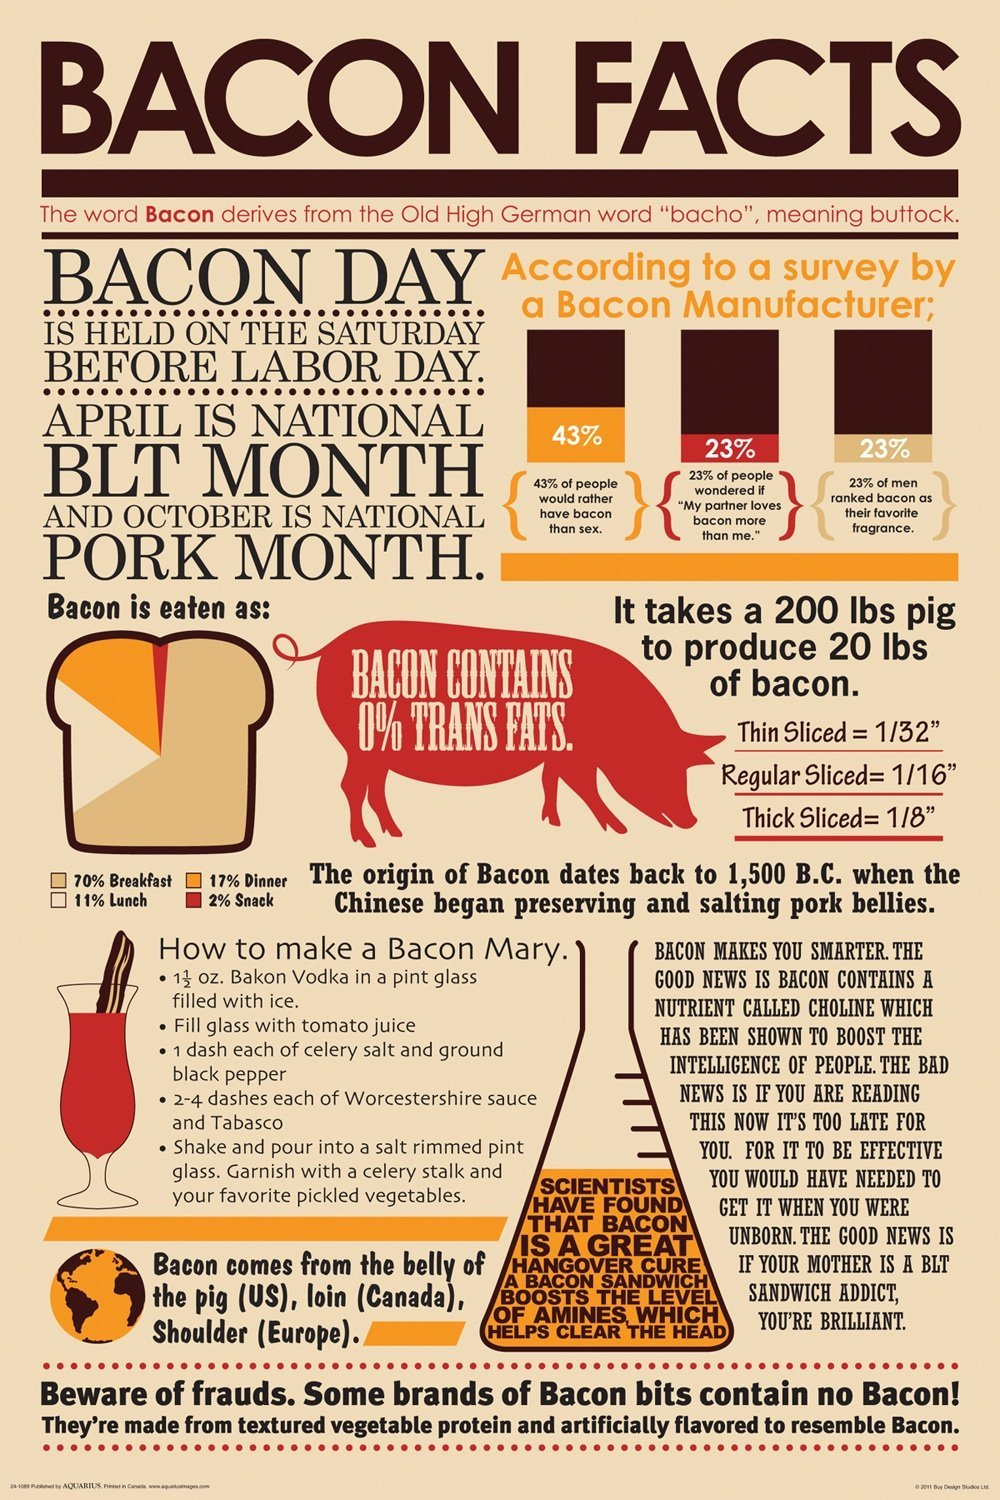
\includegraphics[width=0.5\linewidth]{img/tableDetection/readingOrderIssue.jpg}
\caption{Reading order problems. Determination of correct labels is sometimes hard even for human perception.} \label{fig:readingOrderProblems}
\end{figure}

\begin{figure}[t]
\centering
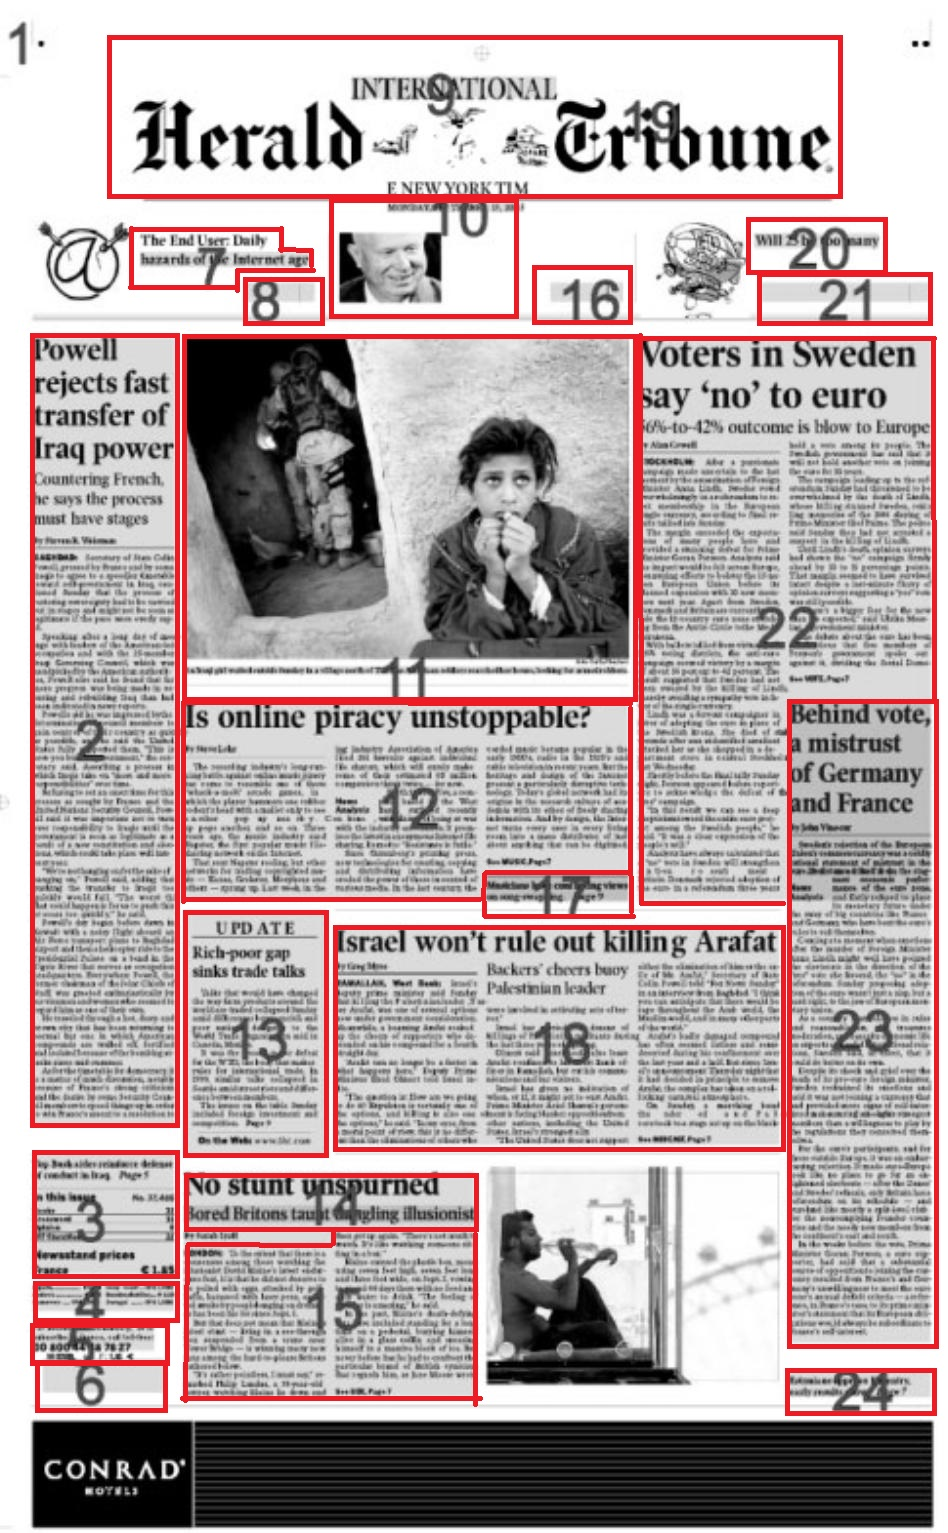
\includegraphics[width=0.5\linewidth]{img/tableDetection/readingOrder.jpg}
\caption{An example of layout analysis~\citep{hadjar2004xed}.}
\label{fig:readingOrderExample}
\end{figure}

Various heuristics are used for the determination of labels~\cite{logicalLayoutTemplate}. In the following list, we overview several of the most widely used:

\begin{itemize}
\item[\emph{Templates}]

The most simple and basic approach is the technique of the already mentioned templates. It is based on a limited number of predefined document layouts (\emph{templates}), which already contain the information about the structure of individual elements. An input document is then matched to these layouts. In the OCR engines that focus solely on processing a single type of documents (such as ticket validation, recipe or passport recognition, recognition of forms filled out by patients in hospitals), this process yields almost perfect results, even though it is a naive approach.

\item[\emph{Rule-based approaches}]

A human reader often determines the logical succession of document elements by font settings and locations of the elements. Rule-based approaches take advantage of this fact and create heuristic ``rules'' that determine the type of the element. For example, a rule for a page header could be ``has the smallest y-axis value, has font size above 22pt, is bold, and is the only element on its line''.

\item[\emph{Syntactic methods}]

These methods present the structure used for element labeling in a form of a set of formal (usually context free) grammars. These grammars contain rules for aggregating pixels into more structured entities until they form logical objects. Parsers for a syntactic analysis are automatically obtained from these grammars. They are then used to perform the actual labeling of the detected elements.

\item[\emph{Machine learning}]

Already mentioned in this thesis, a non-heuristic approach to logical layout analysis is the use of neural networks. Given enough information and time for training, the networks are able to determine the labeling on their own.

There exist various techniques of machine learning, distinguished by the way the neural networks are trained. For example, a neural network can be given a set of rules and input images, which leads the learning process to produce results similar to human observation. Also, it can be solely reliant on raw physical data and itself.

\end{itemize}

Worth mentioning are also techniques like \emph{Blackboard system}, \emph{Description language} or methods based on \emph{Hidden Markov Models}~\cite{logicalLayoutOther}.

Layout analysis is a crucial part of almost every OCR engine. If either geometric or logical layout analysis fails, the input of the recognition engine might contain corrupted data. This might lead to a significantly lower accuracy of the recognition process. 

Table recognition utilizes the output of layout analysis and extracts table related information, such as table cells, headers and footers, from it. Other elements are discarded (e.g. floating text, graphics), as they are considered worthless for the purposes of table recognition.

\section{Table recognition}

The goal of table recognition is to determine if a table even is present on a page, and if yes, where and what its content is. This process is often divided into two parts --- \emph{table detection} and \emph{table decomposition}, with table detection determining the presence and placement of a table, and table decomposition analyzing its content and producing a meaningful structure of its representation. In our thesis, we approach the table recognition problem as a whole, as usually, both parts benefit from reusing each others outputs.

Although obtaining the elements of a simple $m{\times}n$ grid is an easy task achieved by a simple line detection algorithm (e.g. Hough transform~\cite{houghTransform}), the absence of cell borders requires more complicated heuristics. Moreover, tables that contain cells of different sizes, various numbers of cells in different rows, complicated headers or footers, multi-line cells and many more also require more complex solutions. We present a few of these possible obstacles in~\cref{fig:tableRecognitionObstacles}.

\begin{figure}[t]
\centering
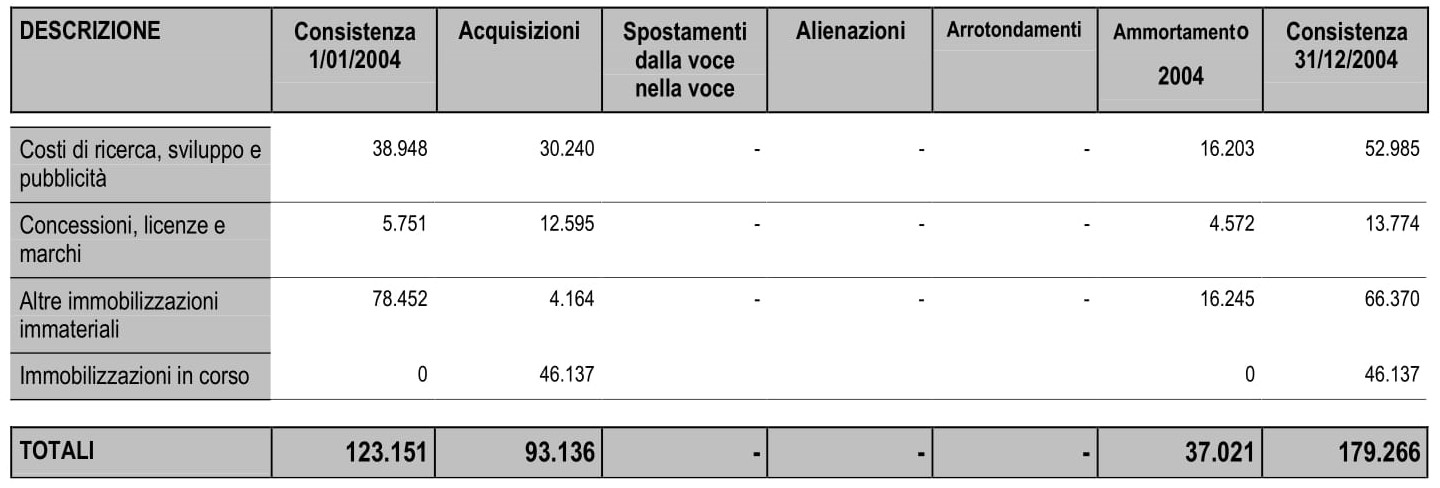
\includegraphics[width=0.7\linewidth]{img/tableDetection/recognitionProblematic.jpg}
\caption{Several common problems occurring during table recognition: missing horizontal and vertical lines; missing information in cells; multi-line cells in the first column and header row; different alignment of header and content cells.}
\label{fig:tableRecognitionObstacles}
\end{figure}

In this section, we overview some of the existing table recognition algorithms. For the purposes of this thesis, we specifically focus on the table recognition implementation of the Tesseract engine.

\subsection{Tesseract table recognition} \label{tableFind}

The Tesseract engine has been originally used for character detection. Over the years, many features have been added, including a \textsc{TableFind} algorithm for table detection and recognition.

\citet{tableDetHeterogeneous} based the TableFind recognition algorithm on already existing Tesseract's features, including layout analysis (described in~\cref{sectionTessPageSegm}) and character detection (\cref{tesseractCharacterRecognition}). Following are the individual steps of the algorithm, along with their visualization in~\cref{fig:tesseractTableRecognition}: 

\begin{enumerate}
\item \emph{Layout analysis}

First, layout analysis is performed by \emph{tab-stop detection}~(\cref{sectionTessPageSegm}) included in the Tesseract library. The results of this step include not only a list of segmented blocks, but also the column layout (~\cref{fig:tessTableDet1}) and column partitions (sequences of connected components of the same type --- like text, image --- that do not cross any tab-line, presented in~\cref{fig:tessTableDet2}).

\item \emph{Identification of table partitions}

With the page layout available, TableFind tries to identify text column partitions that could possibly belong to a table --- \emph{table partitions}. This process is based on heuristics, by identifying column partitions that contain at least one large gap between their connected components, consist of only one word, or overlap with other partitions along the y-axis.

This stage of the algorithm is performed quite aggressively, so although this process returns the desired table partitions, it also produces a lot of false positives, such as considering section headings, page headers, footers, equations, etc., as tables. Most of these unwanted partitions are then removed by a heuristic filter. However, as presented in~\cref{fig:tessTableDet3}, the presence of minor mistakes is not completely eliminated.

\item \emph{Detection of table columns}

As shown in~\cref{fig:tessTableDet4}, vertically aligned partitions are grouped into a single column. Columns with only one partition are then removed. 

\item \emph{Table construction}

The goal of table construction is to group table columns into a table. Here, TableFind assumes that flowing text does not share space with a table along the y-axis. Therefore, boundaries of table columns are expanded along the y-axis to the borders of the page columns that contain them. In result, bounding boxes are created for whole tables. Tables that span across multiple page columns are detected only if a table column exists that belongs to all of these page columns.

\item \emph{Removal of false positives}

Because of relatively greedy heuristic used in the previous step, non-tabular content may be falsely identified in a table. Therefore, TableFind finally removes tables with only one column. This produces the final result (\cref{fig:tessTableDet5}).

\end{enumerate}

The algorithm has been proved to have a 86\% precision. The biggest problems have shown to be full-page tables, often resulting in over or under-segmentation, partial detection or detection of false positives~\citep{tableDetHeterogeneous}.

Another problem with TableFind is that currently, there exists no simple command that a user could run to see the output of this algorithm. To actually detect a table, a user must first write its own program that uses the functions of the added Tesseract table recognition files. Then, he needs to process the data the library returns and output them in a meaningful format, which requires a non-trivial knowledge of the Tesseract implementation.

We further present the results of this algorithm in~\cref{resultsTableFind}, where we compare them to our implementation.
   
\begin{figure}
\centering
\begin{subfigure}{0.30\textwidth}
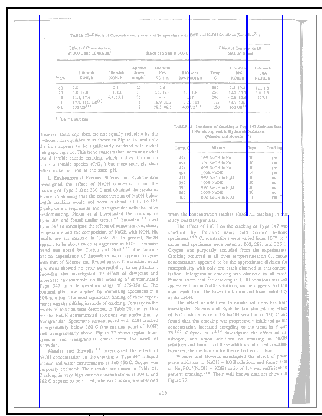
\includegraphics[width=\linewidth]{img/tableDetection/tableDetectionColumns.pdf}
\caption{Column layout.}
\label{fig:tessTableDet1}
\end{subfigure}
\quad
\begin{subfigure}{0.30\textwidth}
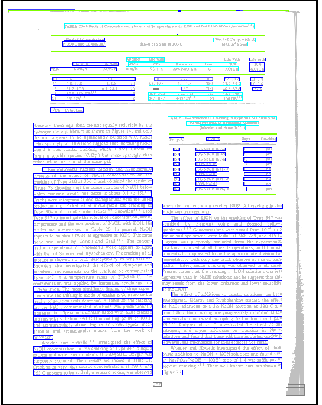
\includegraphics[width=\linewidth]{img/tableDetection/tableDetectionPartitions.pdf}
\caption{Column partitions.}
\label{fig:tessTableDet2}
\end{subfigure}
\quad
\begin{subfigure}{0.30\textwidth}
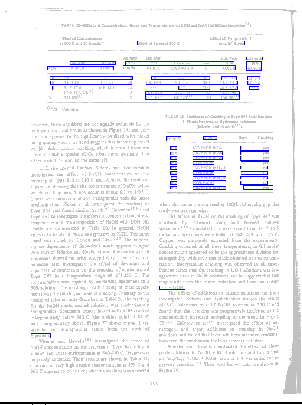
\includegraphics[width=\linewidth]{img/tableDetection/tableDetectionCandidate.pdf}
\caption{Candidate table partitions.}
\label{fig:tessTableDet3}
\end{subfigure}
\\
\begin{subfigure}{0.30\textwidth}
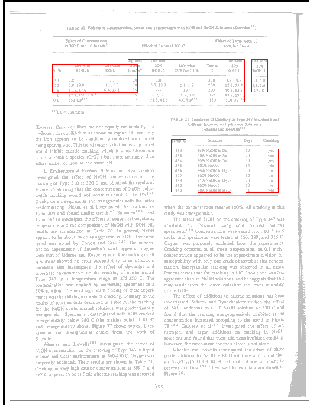
\includegraphics[width=\linewidth]{img/tableDetection/tableDetectionTabCols.pdf}
\caption{Table columns.}
\label{fig:tessTableDet4}
\end{subfigure}
\quad
\begin{subfigure}{0.30\textwidth}
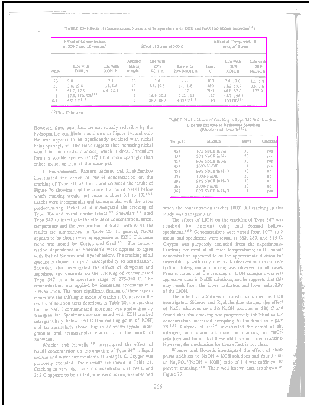
\includegraphics[width=\linewidth]{img/tableDetection/tableDetectionResult.pdf}
\caption{Detected table regions.}
\label{fig:tessTableDet5}
\end{subfigure}
\caption{The process of Tesseract table recognition~\cite{tableDetHeterogeneous}.}
\label{fig:tesseractTableRecognition}
\end{figure}

\subsection{Other existing approaches}

In addition to the TableFind algorithm, there exist various heuristic approaches for table detection. In this section, we overview several of them, including their advantages and disadvantages. Specifically, we focus on T-Recs table recognition system~\citep{TRecs}, Medium-independent table detection~\citep{MediumTable}, pdf2table project~\cite{pdf2table} and an approach based on a hierarchical MXY tree page representation~\citep{tableDetectCesarini}. However, multiple other approaches also exist. Worth mentioning is also, for example, sparse line detection~\cite{sparseLineDetection}, which already uses principles of machine learning. Some of the other methods are briefly reviewed by~\citet{otherDetection1} or~\citet{otherDetection2}.

One of the first approaches to table recognition was presented by the \emph{T-recs} table recognition system~\cite{TRecs}, which is based on a bottom-up approach of clustering word bounding boxes and building a ``segmentation graph''. This segments the page into different regions, which are then evaluated by certain heuristic criteria for tables. Although widely popular in the 90s, this technique has several setbacks. T-Recs is controlled by a set of numerical parameters, which need to be adjusted manually by the user according to the layout of the page. Moreover, it yields unsatisfactory results on multi-column documents.

Another algorithm was described by~\citet{MediumTable}. In single-column documents, a page can be easily segmented into individual textlines. The table detection problem is then perceived as an optimization problem, where the start and end textlines that belong to a table are identified by optimizing some quality function. However, this approach fails on multi-column documents, and on documents that contain more than one table.

\citet{tableDetectCesarini} describe an approach based on hierarchical MXY-tree-like representation. The presence of a table is determined by searching the tree for parallel lines that contain white spaces, and other perpendicular lines between them, which indicate cell borders. Located tables are merged on the basis of proximity and similarity criteria. However, this approach fails if no lines in tables are present.

Method presented by the \emph{pdf2table} project~\cite{pdf2table} is based on assigning each text object of the page its positional attributes. By the evaluation of these attributes, text objects are then merged into single-lines (lines with only one text object), multi-lines (lines with more than one text object) and multi-line blocks (multiple multi-lines merged together). The table detection algorithm then merges the multi-line blocks that may belong to the same table, with the help of a heuristic threshold that determines the greatest number of single-line objects between two multi-line blocks possible. This method also assumes the input to be a single-column document. Despite of that, the user can manually adjust the information about the number of columns, which yields more accurate results.
\chapter{Table recognition implementation}

This chapter gives us an overview of procedures and tools used to create a table recognition software. 

The project is written in C++ and compilable using CMake (tested on MSVC~2017 and g++~7.4). We chose CMake for its cross-platform support and its ability to work with external dependencies (e.g. Tesseract, Leptonica). 

The implementation is divided into two main parts --- \emph{preprocessing}, which prepares the input images for recognition, and \emph{tabular OCR}, which applies our heuristic algorithm for table recognition. Both parts use the features of the Leptonica library and tabular OCR utilizes the character and textline recognition of the Tesseract engine. The image processing in the program is schematized in~\cref{fig:programFlow}.

\begin{figure}
    \centering
	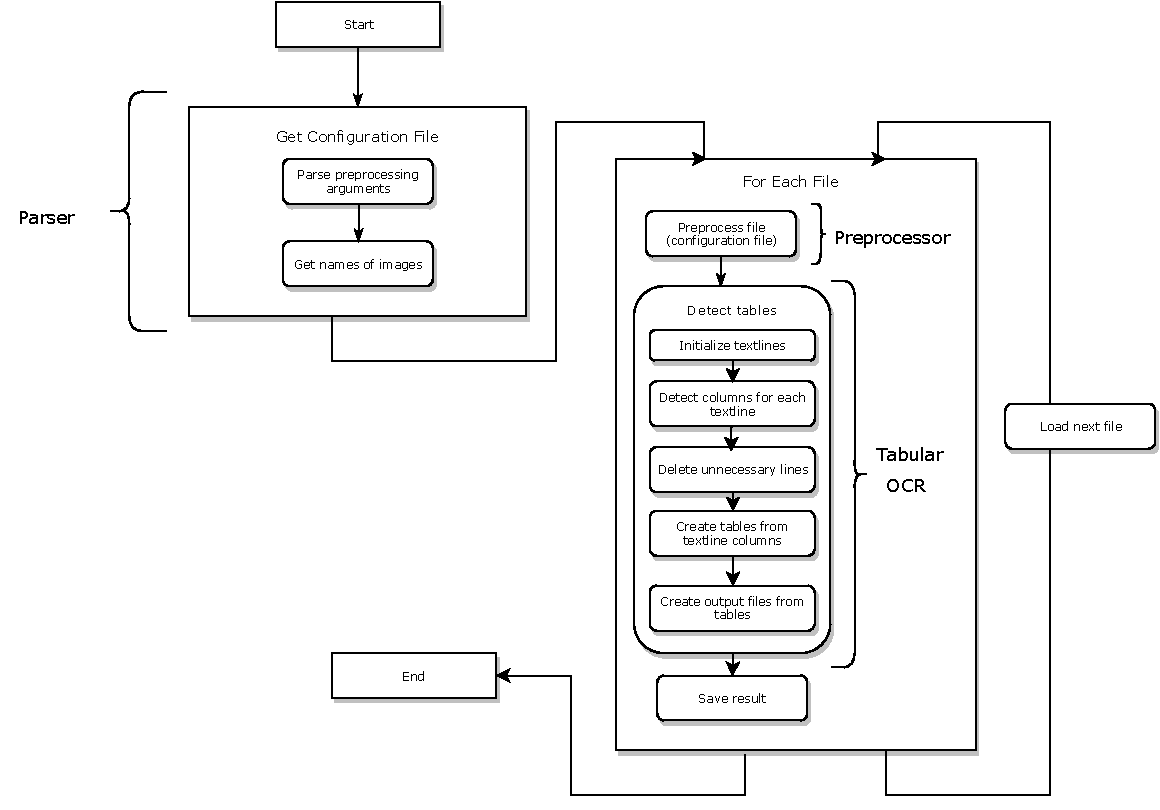
\includegraphics[width=1.0\linewidth]{img/implementation/programFlow.pdf}
	\caption{Program flow diagram}
	\label{fig:programFlow}
\end{figure}

\section{Preprocessing}

The preprocessing part is basically a wrapper around the Leptonica library. Based on the input arguments of our software, the preprocessor calls relevant Leptonica's methods with specified parameters. Not all of the Leptonica's preprocessing features are currently supported in our implementation. However, it is a simple task to add the rest of them. Currently supported methods are the following:

\begin{itemize}
    \item \emph{Contrast enhancement}, specifically histogram equalization (mentioned in~\cref{contrastEnhancemet}), a method of non-linear stretching called gamma correction~\cite{rahman2016adaptive}, and a simple method of linear stretching based on an arctangent function.
    \item \emph{Greyscale conversion}, specifically the averaging technique and luma correction technique (both mentioned in~\cref{grayscaleConversion}). Supported are also two techniques from the Leptonica library based on the selection of either the maximal or minimal value from the three RGB components.
    \item \emph{Binarization}, specifically the support of Otsu and Sauvola binarization techniques, both mentioned in~\cref{binarization}.
    \item \emph{Deskewing}, which does not contain any options. This is due to the fact that Leptonica contains only one deskewing function, which is based on the calculation of projection profiles ( mentioned in~\cref{deskewing}) with the help of Hough transform~\cite{bloomberg2analysis}.
\end{itemize}

The initial idea for preprocessing was to provide more complex functions which are included in the OpenCV library. However, this was not the goal of the thesis. Therefore, the preprocessing part stayed very simple and mostly demonstrative and the user is still advised to preprocess the images manually.

\section{Tabular OCR}

After the preprocessing part is done, the preprocessed image is passed to tabular OCR for table recognition. The individual steps of our heuristic table recognition algorithm are executed in the main \texttt{process\_image} function.

In this section, we analyze this algorithm step-by-step and overview the functions used. During the process, we use the concept of \emph{textlines} --- rows of the image document that contain recognized character symbols.

Our algorithm is based on the already mentioned Tesseract symbol and textline recognition~\cref{tesseractCharacterRecognition} and moreover on whitespace detection. Upon detecting whitespaces between individual symbols, we try to heuristically estimate the whitespaces between words and, furthermore, columns, for each textline of the image. Once we have all the textlines separated into columns, we try to merge consecutive lines with similar column layout into a table.  

Following are the individual steps of the algorithm, also visualized in~\cref{fig:implemTableRecogniton}:
\begin{enumerate}
\item \emph{Textline initialization}, which includes the Tesseract recognition process, and from its output obtains all the required information about individual textlines.
\item \emph{Deletion of unnecessary lines}, which removes textlines with no valuable information (e.g. textlines with no symbols, false positives).
\item \emph{Column detection}, which determines the column segmentation for each existing textlines.
\item \emph{Column merge into tables}, which merges the existing columns of textlines into a table.
\item \emph{Output determination}, which processes the information in each recognized table and outputs it in a meaningful structure.
\end{enumerate}

\subsection{Textline initialization} \label{textlineInitialization}

The whole process begins with the detection of individual characters and their merge into textlines (\cref{fig:implem1}). These textlines are then used during the whole process of the algorithm, and are later searched for words, columns etc.

For the purposes of the character recognition, we use the Tesseract engine. We initialize the Tesseract API without the use of neural networks and obtain both lines and symbols. We decided to not use the neural networks due to the fact that they did not produce as accurate results as simple heuristic recognition at the time of testing. However, their performance may increase over the time. Therefore, this setting might need to be manually changed in the future.

After this step, we do not use the features of the Tesseract engine anymore, and rely solely on our heuristic functions.

The symbols and lines obtained from Tesseract are represented as simple boxes, with the symbols also containing textual information. To gain a more detailed information about individual textlines, we therefore iterate over all the lines and symbols and assign symbols into their lines. The result of this function is therefore a list of all textlines containing the information about their individual symbols, like positioning and their actual character value in UTF8.

This function runs in $O(m\cdot n^2)$. The initial idea for this implementation was to firstly sort both the symbols and lines by their y coordinates (which is simply $O(\log n)$ and $O(\log m)$). The assignment of individual symbols into their lines would then be performed by simply iterating symbols and jumping to another line once the current symbol does not fit in the current line, with the iteration therefore having a $O(m\cdot n)$ time complexity. This would present a significant execution time improvement.

However, a problem occurred with this approach. By default, Tesseract's recognition creates a lot of false positives, including noise recognized as dots, white spaces, and, most importantly, horizontal and vertical lines, like footer or header separators, underlinings of words, table borders etc. These false positives disrupt the reading order of the document, which is a factor that this approach relies on.

Although we tried to remove these false positives (for example, removal of empty characters was trivial and required only checking for symbols that contain no textual information), we found no criterion that would suffice all of these obstacles. Therefore, in our current approach, we chose to sacrifice time complexity in favor of accuracy.

\subsection{Deletion of unnecessary lines}

As already mentioned, Tesseract's textline recognition algorithm may include false positives. In this step, we delete all unnecessary lines (\cref{fig:implem2}), specifically:

\begin{itemize}
\item \emph{Empty lines}

Like horizontal or vertical line segments, borders or other lines that contain no UTF8 symbols are of no use and are therefore removed from the textline list.

\item \emph{Table textlines}

Table textlines are parts of the image that are bordered by visible lines, which usually represent either a table, form or even a graphics image. Tesseract often recognizes these parts as single textlines. These textlines therefore contain multiple other textlines, and are significantly greater in height. We remove them by a simple heuristic based on the comparison of their height and the font of their symbols.
\end{itemize}

We present both cases of unnecessary lines in~\cref{fig:deletionOfLines}.

Once this step of the algorithm is done, we are left only with lines that contain symbols and can be a part of the table.

\begin{figure}
\centering
{\sffamily
\begin{tabular}{cc}
Empty lines & Table textline \\
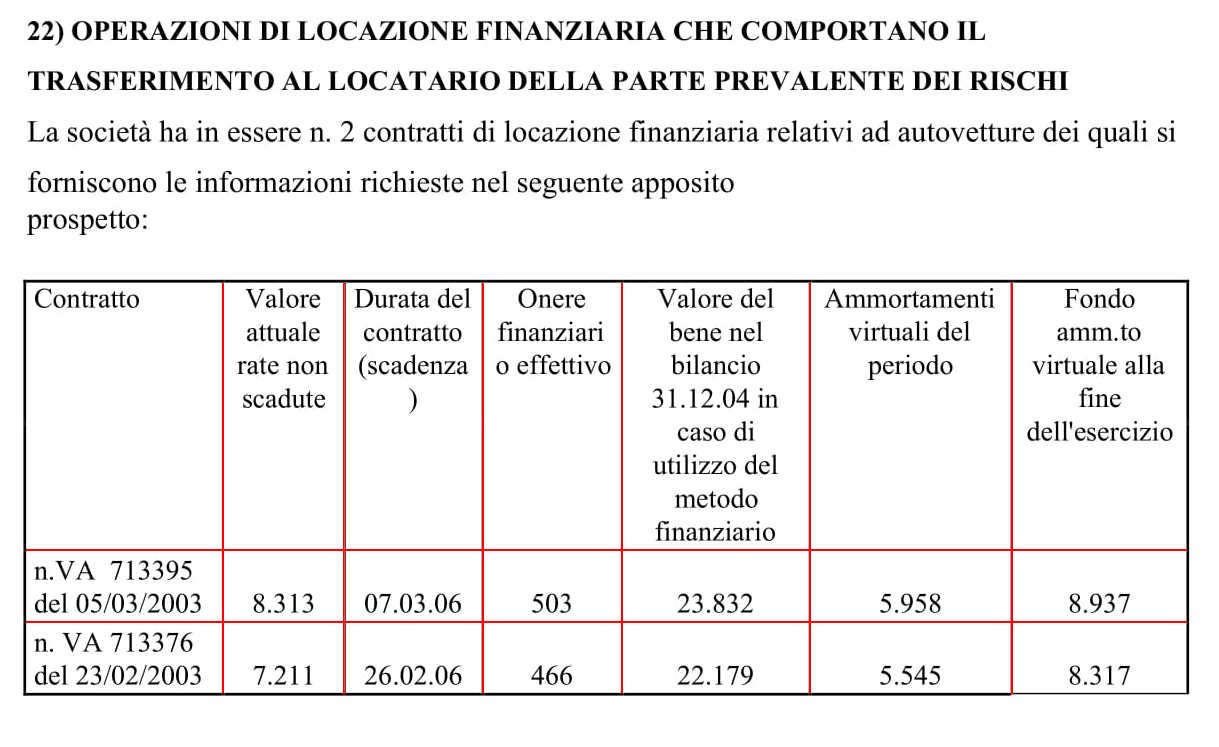
\includegraphics[width=0.4\linewidth]{img/implementation/textlineEmpty.png}
&
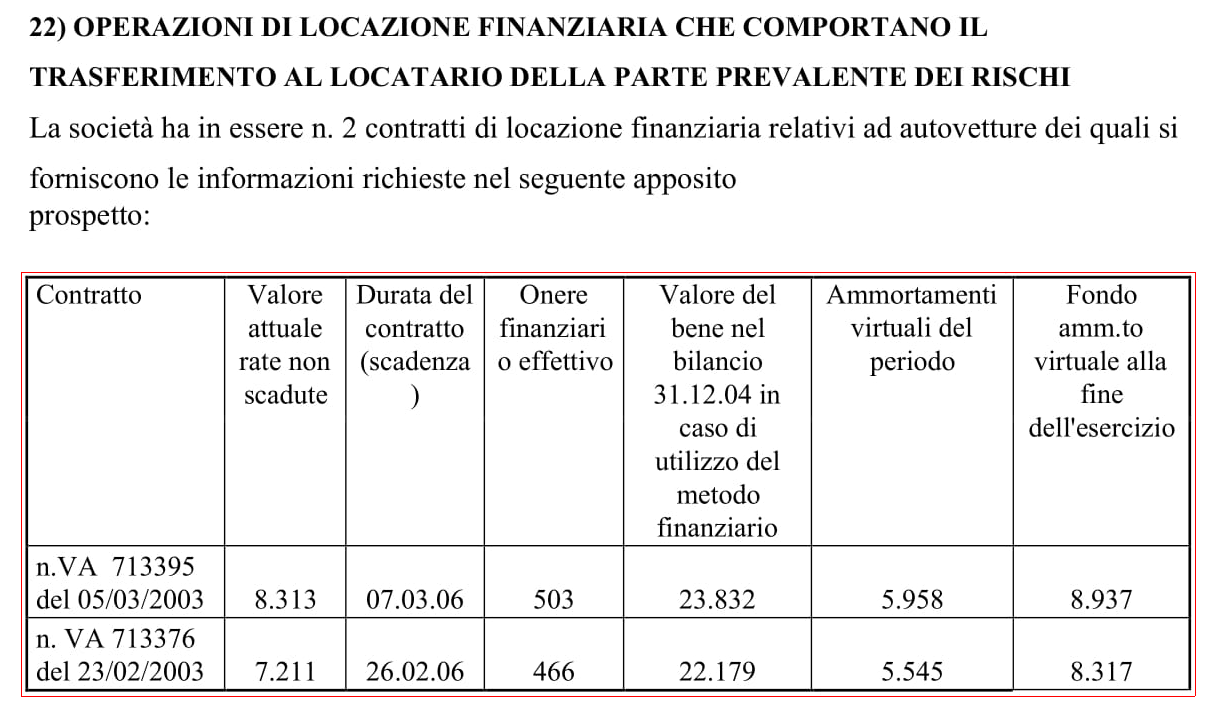
\includegraphics[width=0.4\linewidth]{img/implementation/textlineTable.png}\\
\end{tabular}
}
\caption{Types of unnecessary lines that Tesseract might have recognized as textlines. We remove these lines by heuristic algorithms.}
\label{fig:deletionOfLines}
\end{figure}

\subsection{Column detection} \label{columnDetection}

Upon obtaining individual textlines, we try to determine their segmentation into columns by analyzing the positioning of symbols they contain. This is done for each line individually. Firstly, we merge symbols into words. After that, we merge words into columns (\cref{fig:implem3}). Although we could simply just merge symbols into columns and ignore the whole processing of words, this would leave us with no information about spaces between individual words and would therefore lead to merging of text.

We start this process by obtaining all the spaces between individual symbols and sorting them by size. For human perception, upon seeing this list, to determine the whitespace between individual words and columns is mostly an intuitive and easy task. Following are three lists of spaces. We present the visualized merge of our algorithm according to them in~\cref{fig:symbolMerging}.

\texttt{1 1 2 2 2 3 3 3 3 3 3 3 3 3 3 3 3 4 4 4 4 5 15 15 16 16 18 18 227 235;}

\texttt{2 2 2 2 2 2 2 2 2 3 3 3 3 3 3 3 3 3 3 3 3 4 4 4 4 4 4 4 5 5 6 15 15 16 17 165 235;}

\texttt{1 1 1 2 2 2 3 3 3 3 3 3 3 3 3 3 3 4 4 4 4 4 4 4 4 5 5 15 15 15 17 17 17 18 134 235;}

\begin{figure}
\centering
{\sffamily
\begin{tabular}{c}
The original image \\
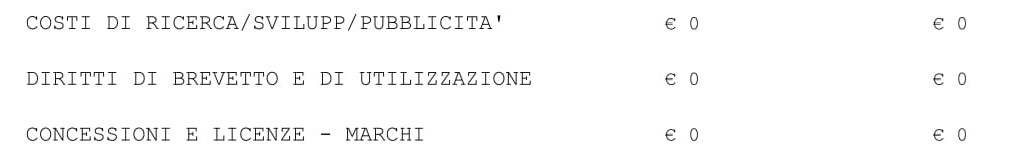
\includegraphics[width=0.8\linewidth]{img/implementation/mergedOrig.jpg}\\
Merged into words \\

\includegraphics[width=0.8\linewidth]{img/implementation/mergedWords.png}\\
Merged into columns \\
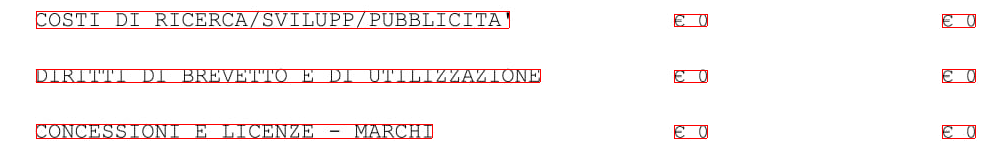
\includegraphics[width=0.8\linewidth]{img/implementation/mergedCols.png}\\
\end{tabular}
}
\caption{The process of merging symbols of a textline.}
\label{fig:symbolMerging}
\end{figure}

It is quite obvious that the word whitespace will therefore be around 5-6 in all cases and column whitespace 227, 165 and 134 respectively. In our implementation, we determine these whitespaces by iterating over all the symbol spaces. Once we find two subsequent spaces that have``sufficiently large difference between their values'', we assume the greater one to be the whitespace between either words, columns or both.

The sufficient difference between subsequent values is based on a calculation of a so-called \emph{multiplication factor}. The whitespace value is then determined according to the code snippet presented in~\cref{whitespaceDetermCode}.

\begin{figure}
{\small \begin{verbatim}
for (it; it != all_spaces.end() - 1; it++)
{
  // get multiplication factor of current space
  double multi_factor = get_multi_factor_words(*it, constant);
  if (*std::next(it) >= multi_factor * *it)
  {
    // found the word whitespace at *std::next(it)
    // code to execute once the whitespace is found
  }
}
\end{verbatim}}
\caption{The code used for the determination of the word whitespace. Column whitespace is determined similarly.}
\label{whitespaceDetermCode}
\end{figure}

From the results of the detection of spaces between individual symbols, we observed that the greater the current space is, the less the multiplication factor should be. Based on this, we have tried many different values and curves for the determination of the multiplication factor. First observations from these attempts led to the estimation that the best curve to use would be logarithmic. However, the current implementation seemed to worked well enough and was therefore left as it is.

The determination of the column whitespace was based on a similar idea with slightly altered parameters.

Upon determining the column and word whitespaces, we then merge symbols by these whitespaces into words and columns respectively.

The determination of whitespaces was probably the most difficult part of the algorithm. There have been multiple different ideas for the implementation. The one that has been preferred most of the time was the idea of separating textlines according to their font sizes. The ones with similar fonts were assigned to the same \emph{font category}, and the whitespace was then determined for the whole category. The word whitespace recognition worked slightly better with this approach. However, the determination of columns had a higher chance of failure, as the sizes of column spaces differed greatly and the algorithm encountered problems when finding the point where word spaces ended and column spaces started. Therefore, the current simpler approach was chosen.

Another initial idea was to simply determine the size of the column space by a constant, e.g. word\_whitespace*constant = column\_whitespace. Surprisingly, the results of this approach were comparable to those of the current implementation. However, it was deemed to fail when it came to small fonts or full-page tables, and had no room for improvement in contrast to the current approach.

\subsection{Column merge into tables}

Once we have the information about columns for each textline, we can start searching for tables. The table detection algorithm is performed by a simple $O(n)$ algorithm by iterating the textlines from top to bottom and merging two consecutive textlines with a similar column layout. The determination of whether two textlines have similar column layout is performed according to~\cref{alg:tableMerge}.

Merge of the textlines is performed by merging the columns that have been detected to overlap, and adding other columns with no such attribute. In a typical $m{\times}n$ table, every column should overlap with the one underneath it, which is also mostly the case when running this algorithm.

Once we have at least two merged textlines, we use this new merged line as a current textline. Therefore, when creating a table, we append new lines to the already merged ones. At the end of this algorithm, our current table is therefore represented as a textline with the information about its columns (and a list of textlines that are in the current table).

\xxx{sformatovat algoritmus}

\begin{algorithm}[p]
\caption{Are textlines in same table}
{\scriptsize
\label{alg:tableMerge}
\begin{algorithmic}
\Require iter\_first \Comment represents the current place we are when iterating over columns of first line
\State iter\_second \Comment represents the current place we are when iterating over columns of second line
\While{true}
\If {either $iter\_first$ or $iter\_second$ is at the end of their line}
\If {at least one pair of columns was found that should be merged}
\State \emph{merge}
\EndIf
\State \emph{break}
\EndIf
\If {current columns overlap} \Comment{a function that checks whether the bounding boxes of the two columns overlap in the x-axis}
\If {found columns do not overlap with other existing columns in the x-axis}
\State save the position of overlapping columns for future merging
\EndIf
\Else 
\State increase either $iter\_first$ or $iter\_second$ depending on which is pointing to the box that has a lower x-axis
\State continue
\EndIf
\State $iter\_first \gets iter\_first+1$
\State $iter\_second \gets iter\_second+1$
\EndWhile
\end{algorithmic}}
\end{algorithm}

\subsection{Output determination}

What we focus on when creating an output are table cells. We create them by simply overlaying rows and columns and saving their common areas as cells. The problem arises with the existence of multi-line rows, that is, rows that often span over multiple textlines. In our implementation, a simple constant-based algorithm is added to recognize at least some of them and therefore merge multiple textlines into one row.

Once we obtain the cells, the only thing left is to create a user-friendly representation of the recognized data. Here, the user has two options according to the parameter he sets in the command line environment. 

The first option is a simple image output. Recognized cells are therefore bordered by colored boxes (\cref{fig:implem4}) in the original input image and saved in a PNG file.

The other option is a JSON structure of the recognized cells, which also contains text within each cell. The JSON structure is demonstrated in~\cref{fig:jsonout}.

\begin{figure}[p]
\lstset{
    string=[s]{"}{"},
    stringstyle=\color{blue},
    comment=[l]{:},
    commentstyle=\color{black},
    basicstyle=\scriptsize
}
\begin{lstlisting}
{"all_tables": {
  "cols": number of columns,
  "rows": number of rows,
  "table_repres": {
    "h": height of table,
    "w": width of table,
    "x": the x-coordinate where the table starts,
    "y": the y-coordinate where the table starts
  },
  "cells": [
        {
        "box": {
           "h": height of current cell,
           "w": width of current cell,
           "x": the x-coordinate where the cell starts,
           "y": they y-coordinate where the cells starts
        },
        "cols_no": in which column of the table the cell is,
        "rows_no": in which row of the table the cell is,
        "text": the UTF8 text displayed in the cell
        },
        ...
        other cells
    ]
  }
  ...
  other tables
}
\end{lstlisting}
\caption{A JSON structure used for the representation of tables recognized from an input image.}
\label{fig:jsonout}
\end{figure}

By default, both output options are selected and therefore two files are saved in the newly created \emph{results} directory inside the build directory.

\begin{figure}[p]
\begin{subfigure}{0.45\textwidth}
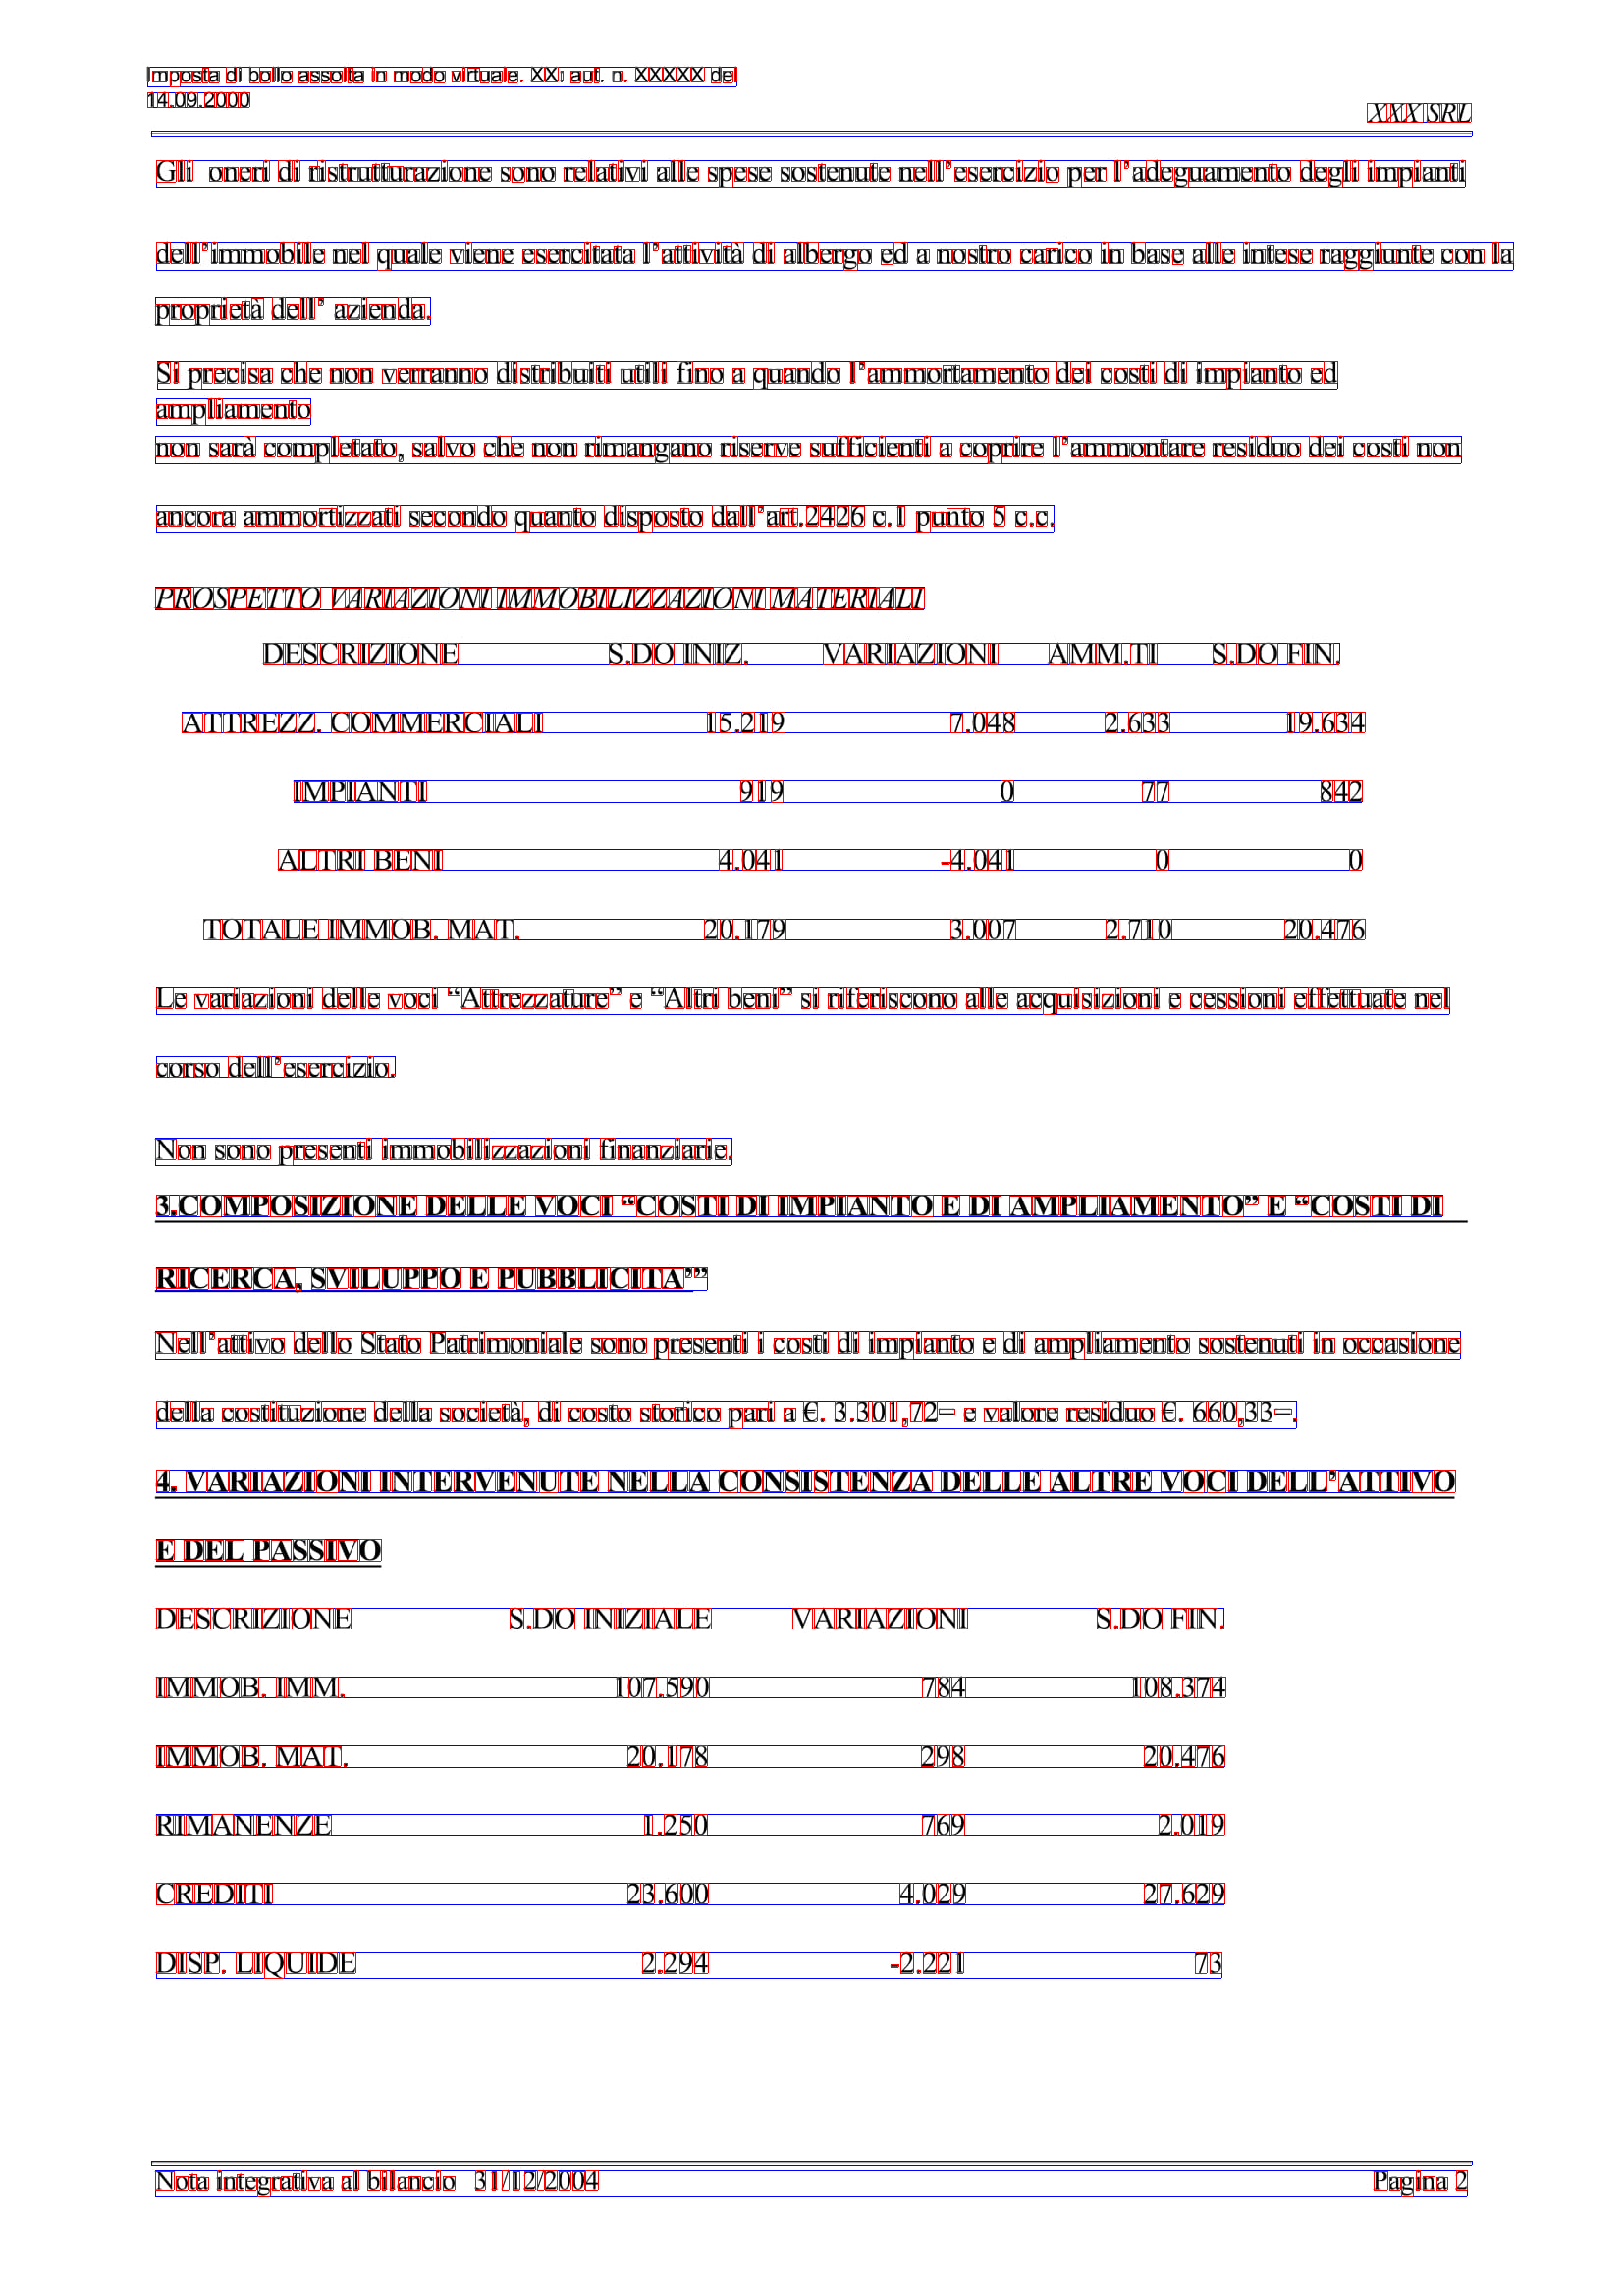
\includegraphics[width=\linewidth]{img/implementation/implem1.png}
\caption{Recognized textlines (blue) and their symbols (red) by the Tesseract recognition. These are merged so the symbols are assigned to their textlines.}
\label{fig:implem1}
\end{subfigure}
\qquad
\begin{subfigure}{0.45\textwidth}
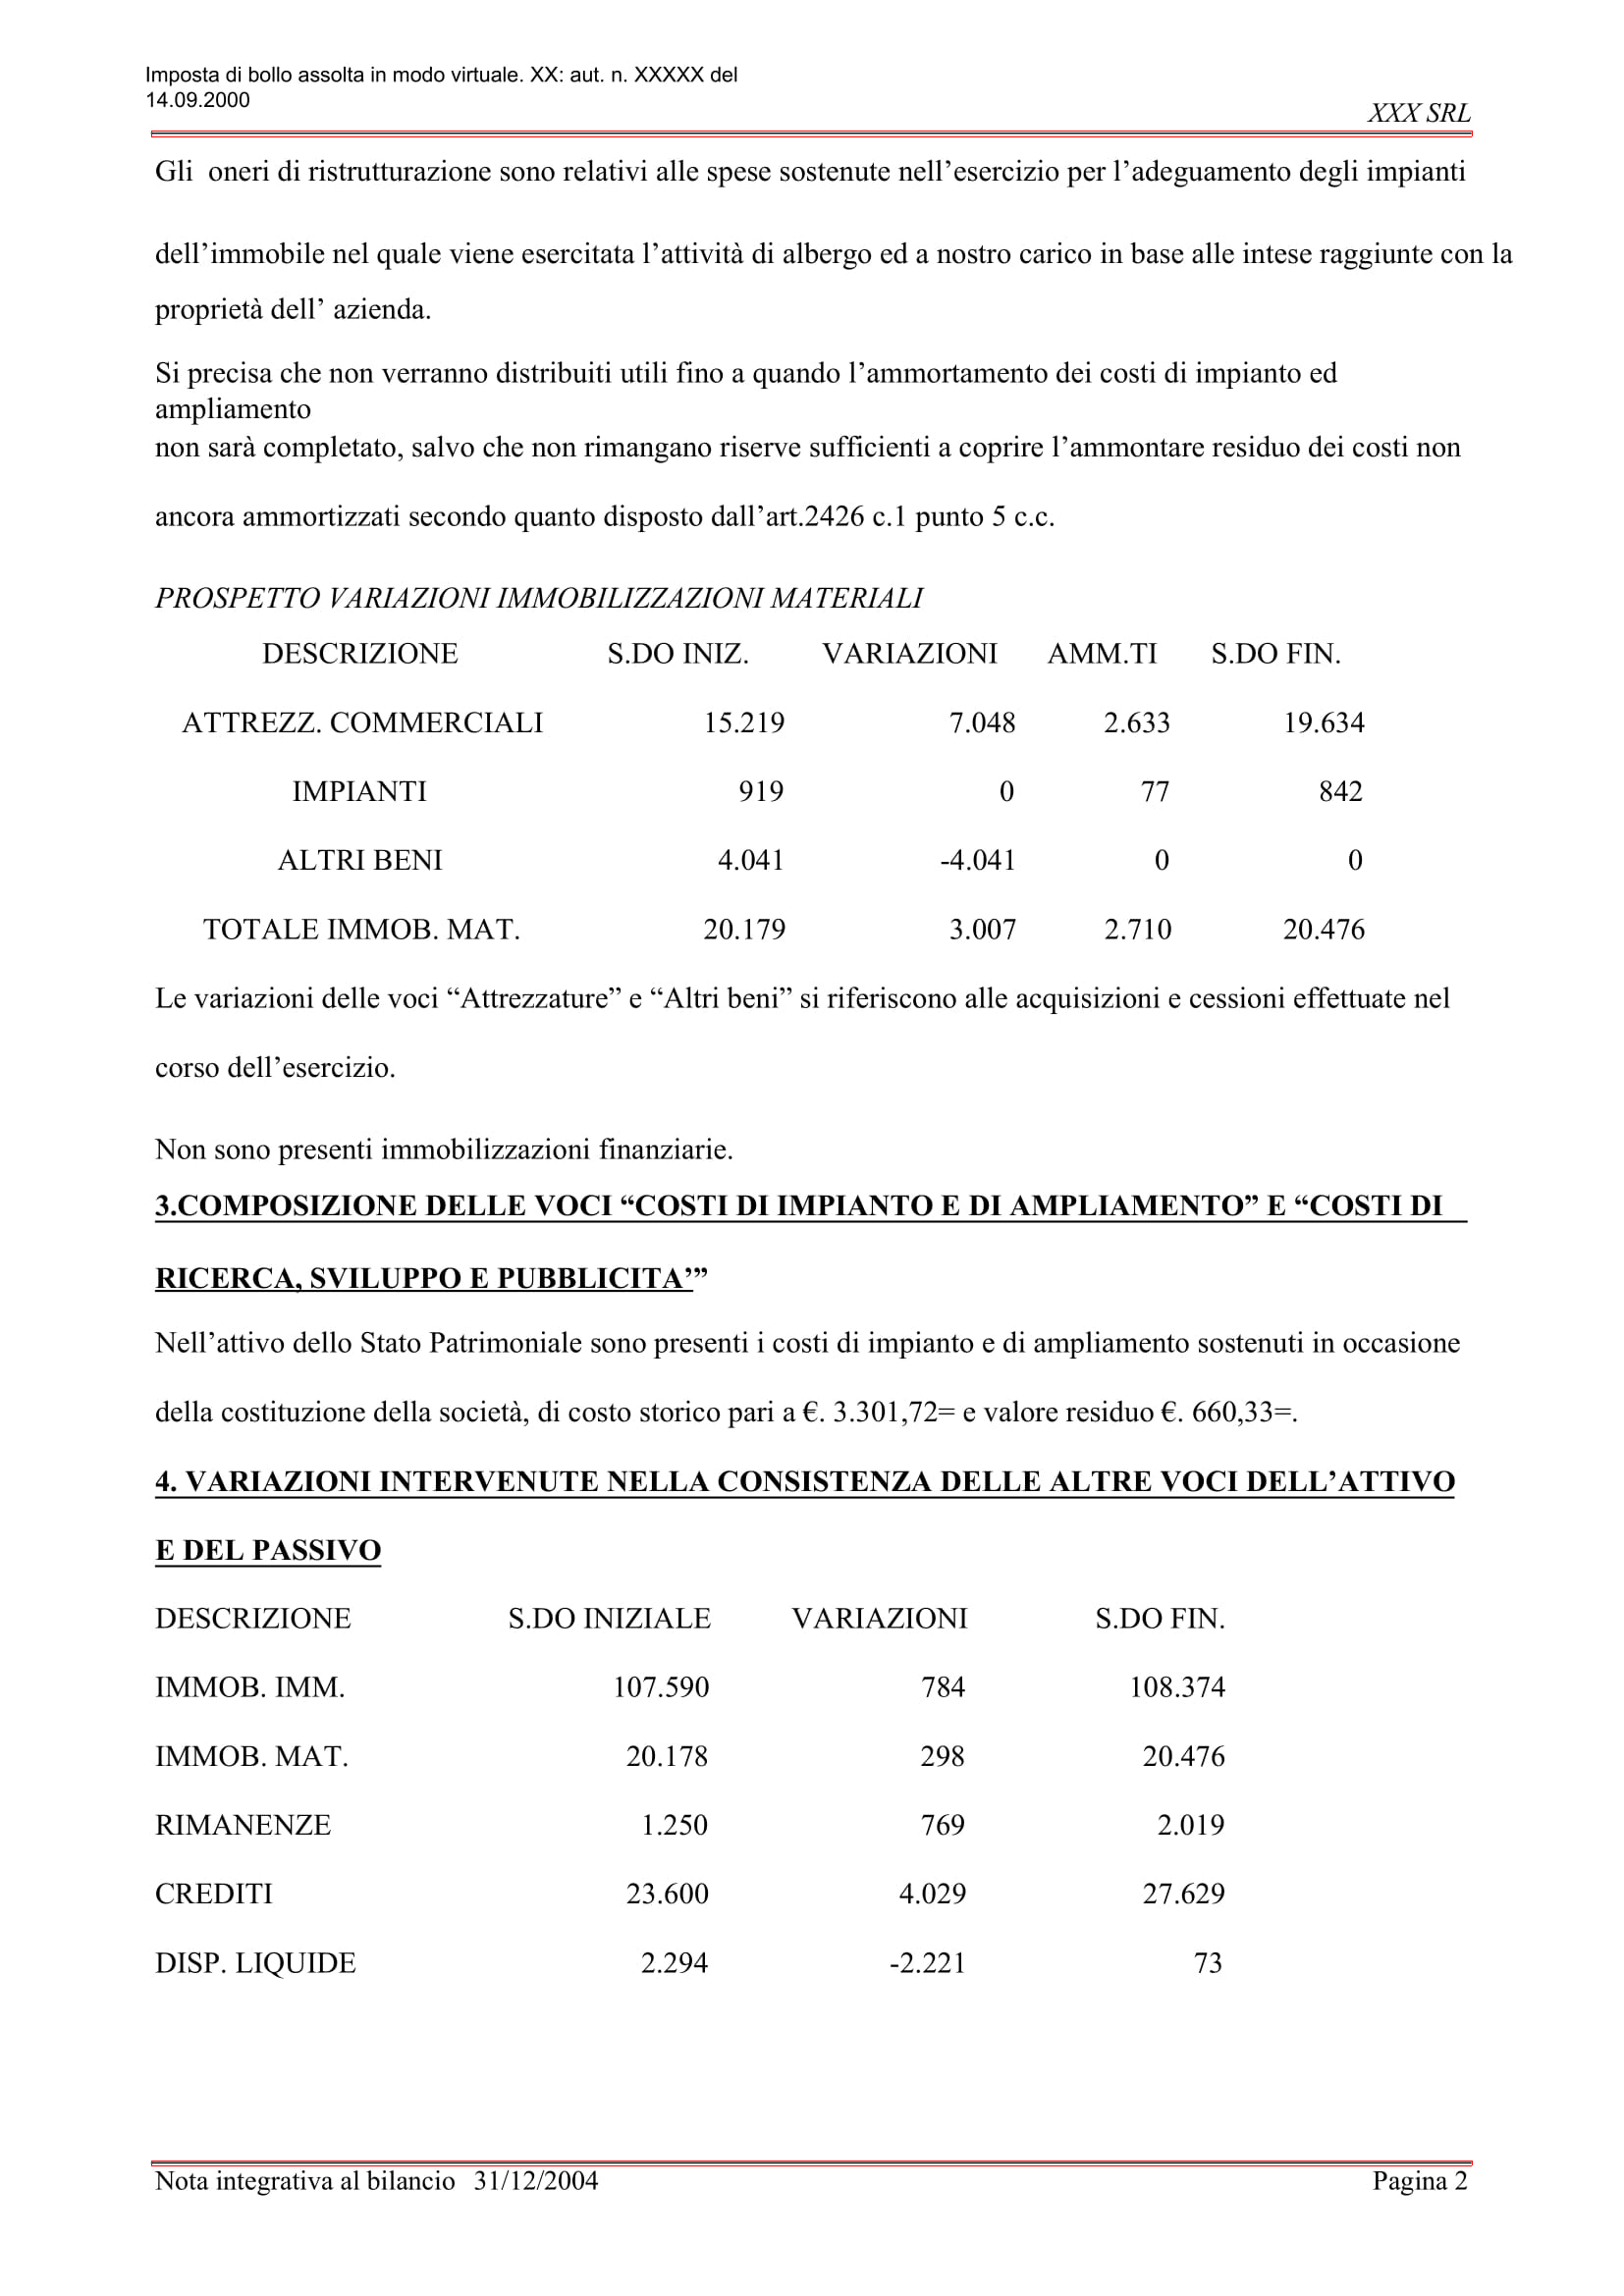
\includegraphics[width=\linewidth]{img/implementation/implem2.png}
\caption{Unnecessary lines recognized from the image. These are removed in this step.}
\label{fig:implem2}
\end{subfigure}
\begin{subfigure}{0.45\textwidth}
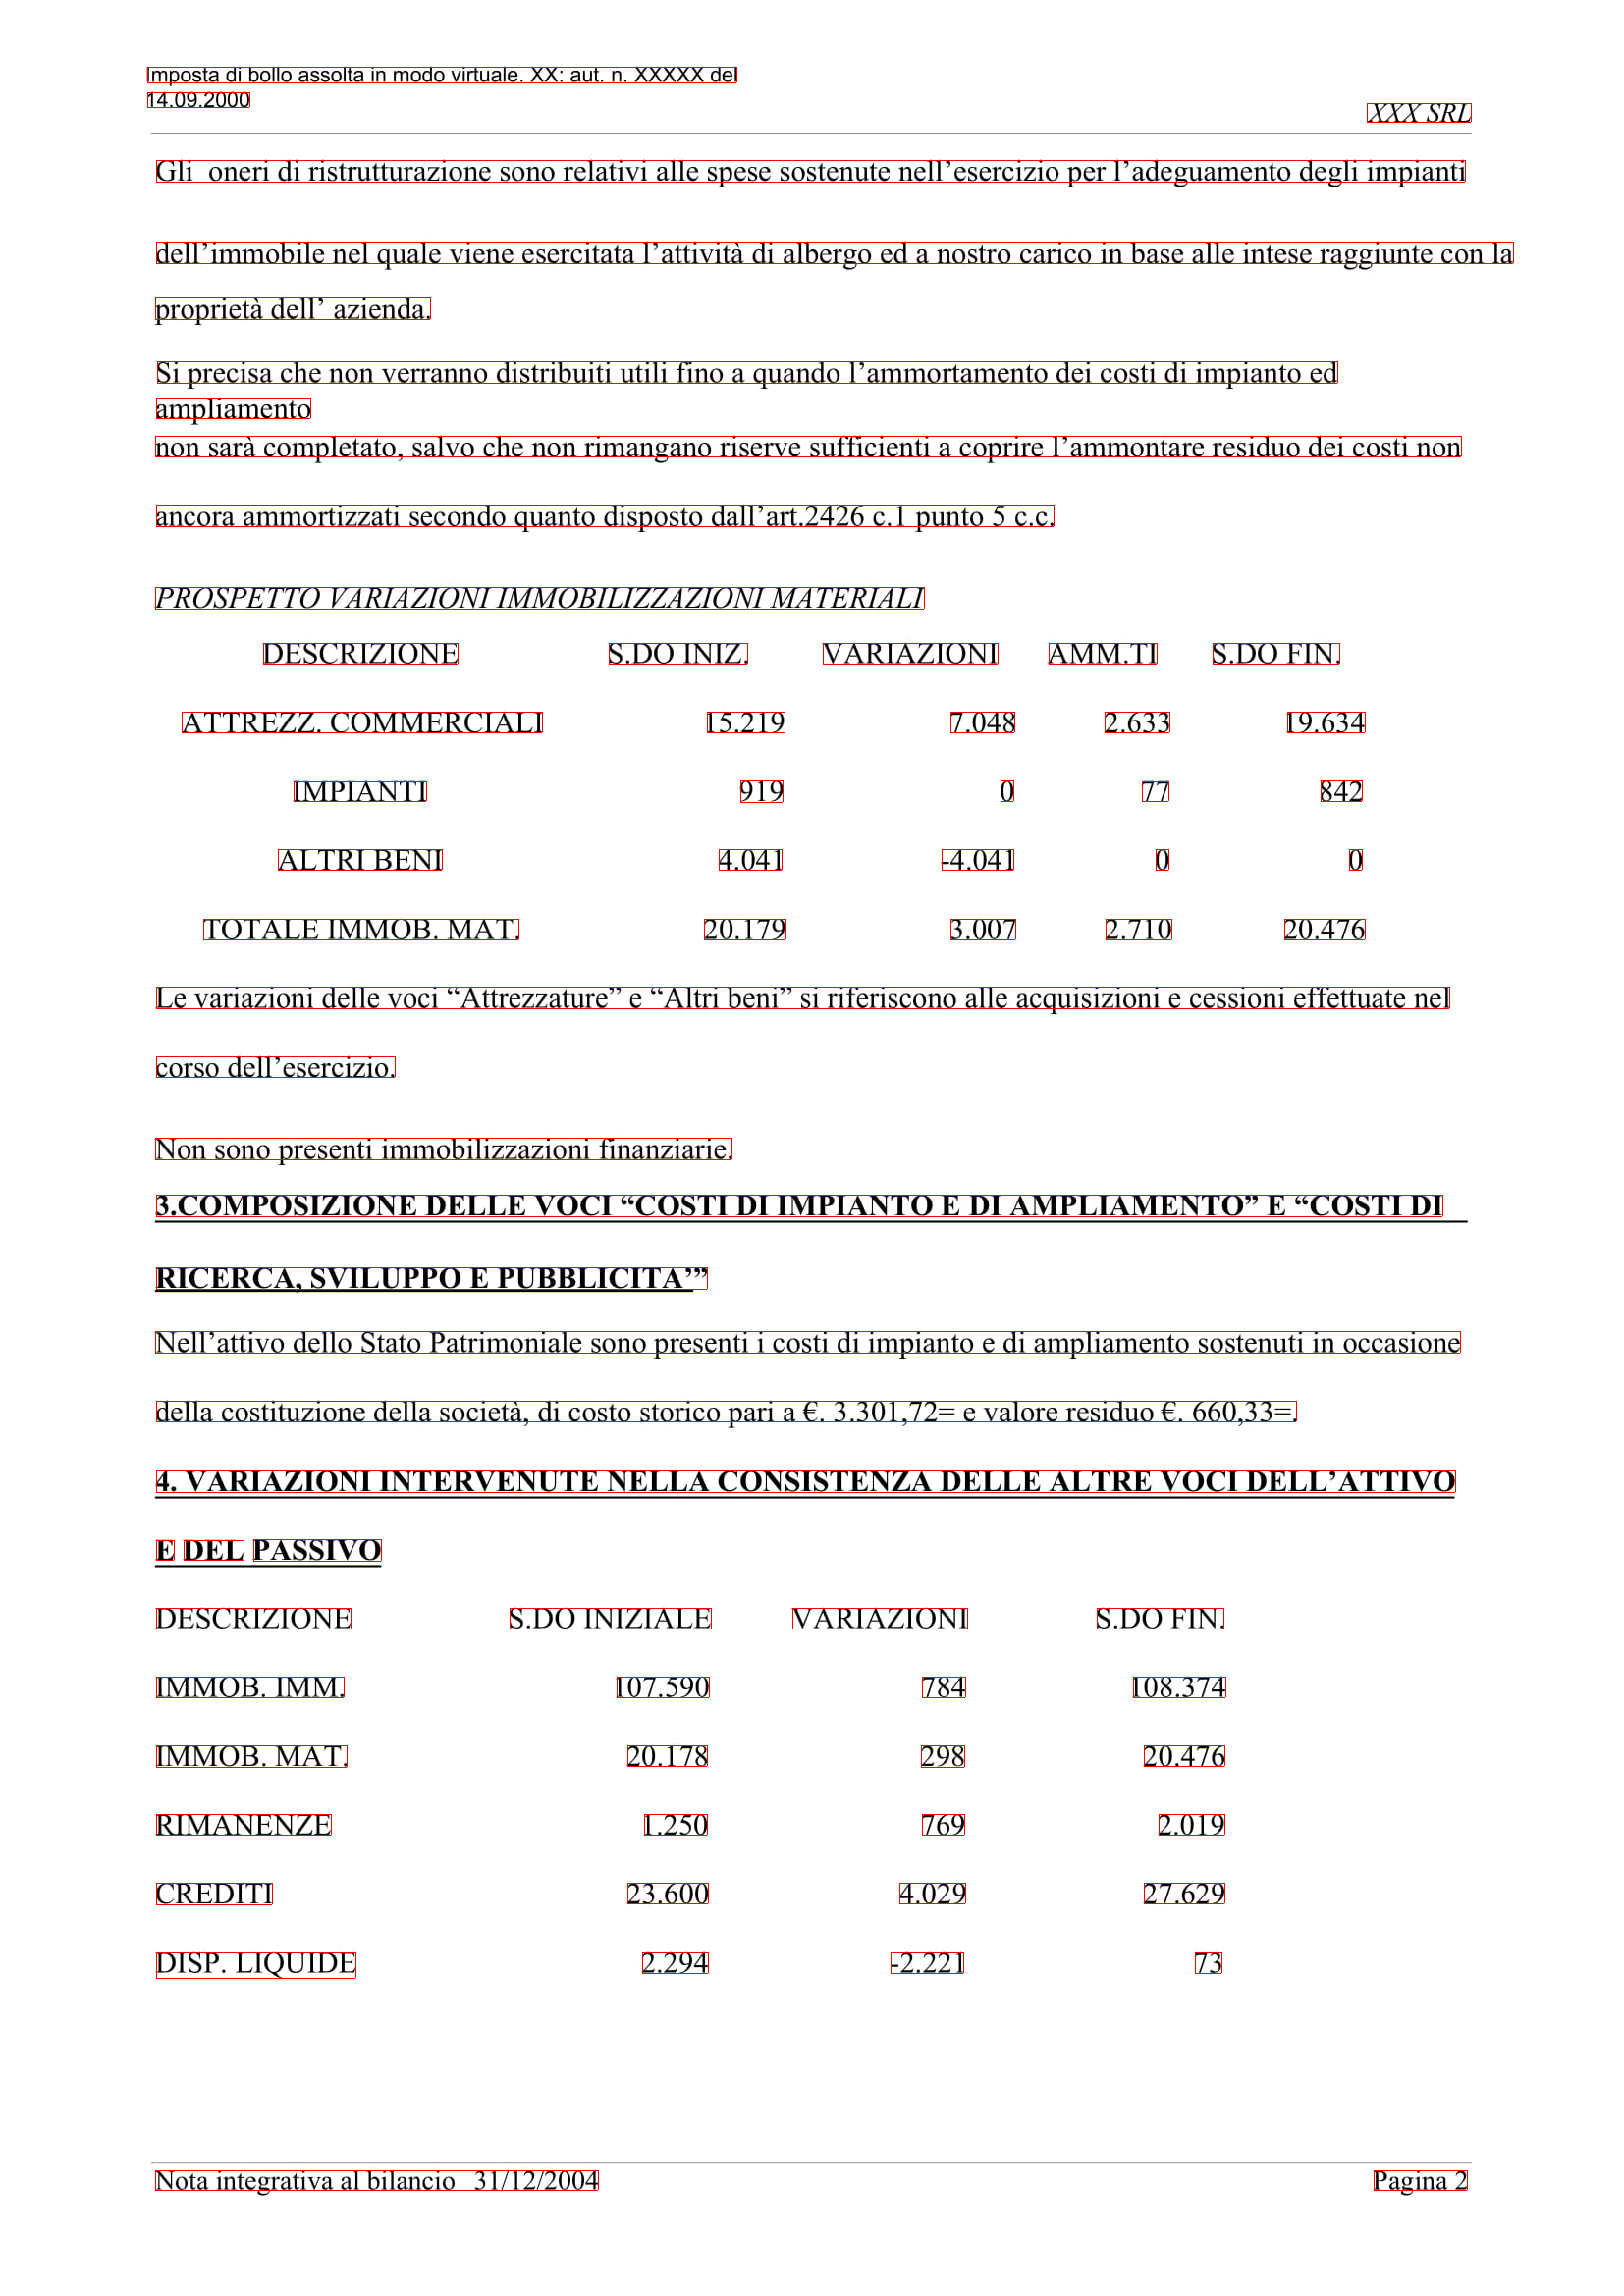
\includegraphics[width=\linewidth]{img/implementation/implem3.png}
\caption{The results of segmentation of each textline into columns.}
\label{fig:implem3}
\end{subfigure}
\qquad
\begin{subfigure}{0.45\textwidth}
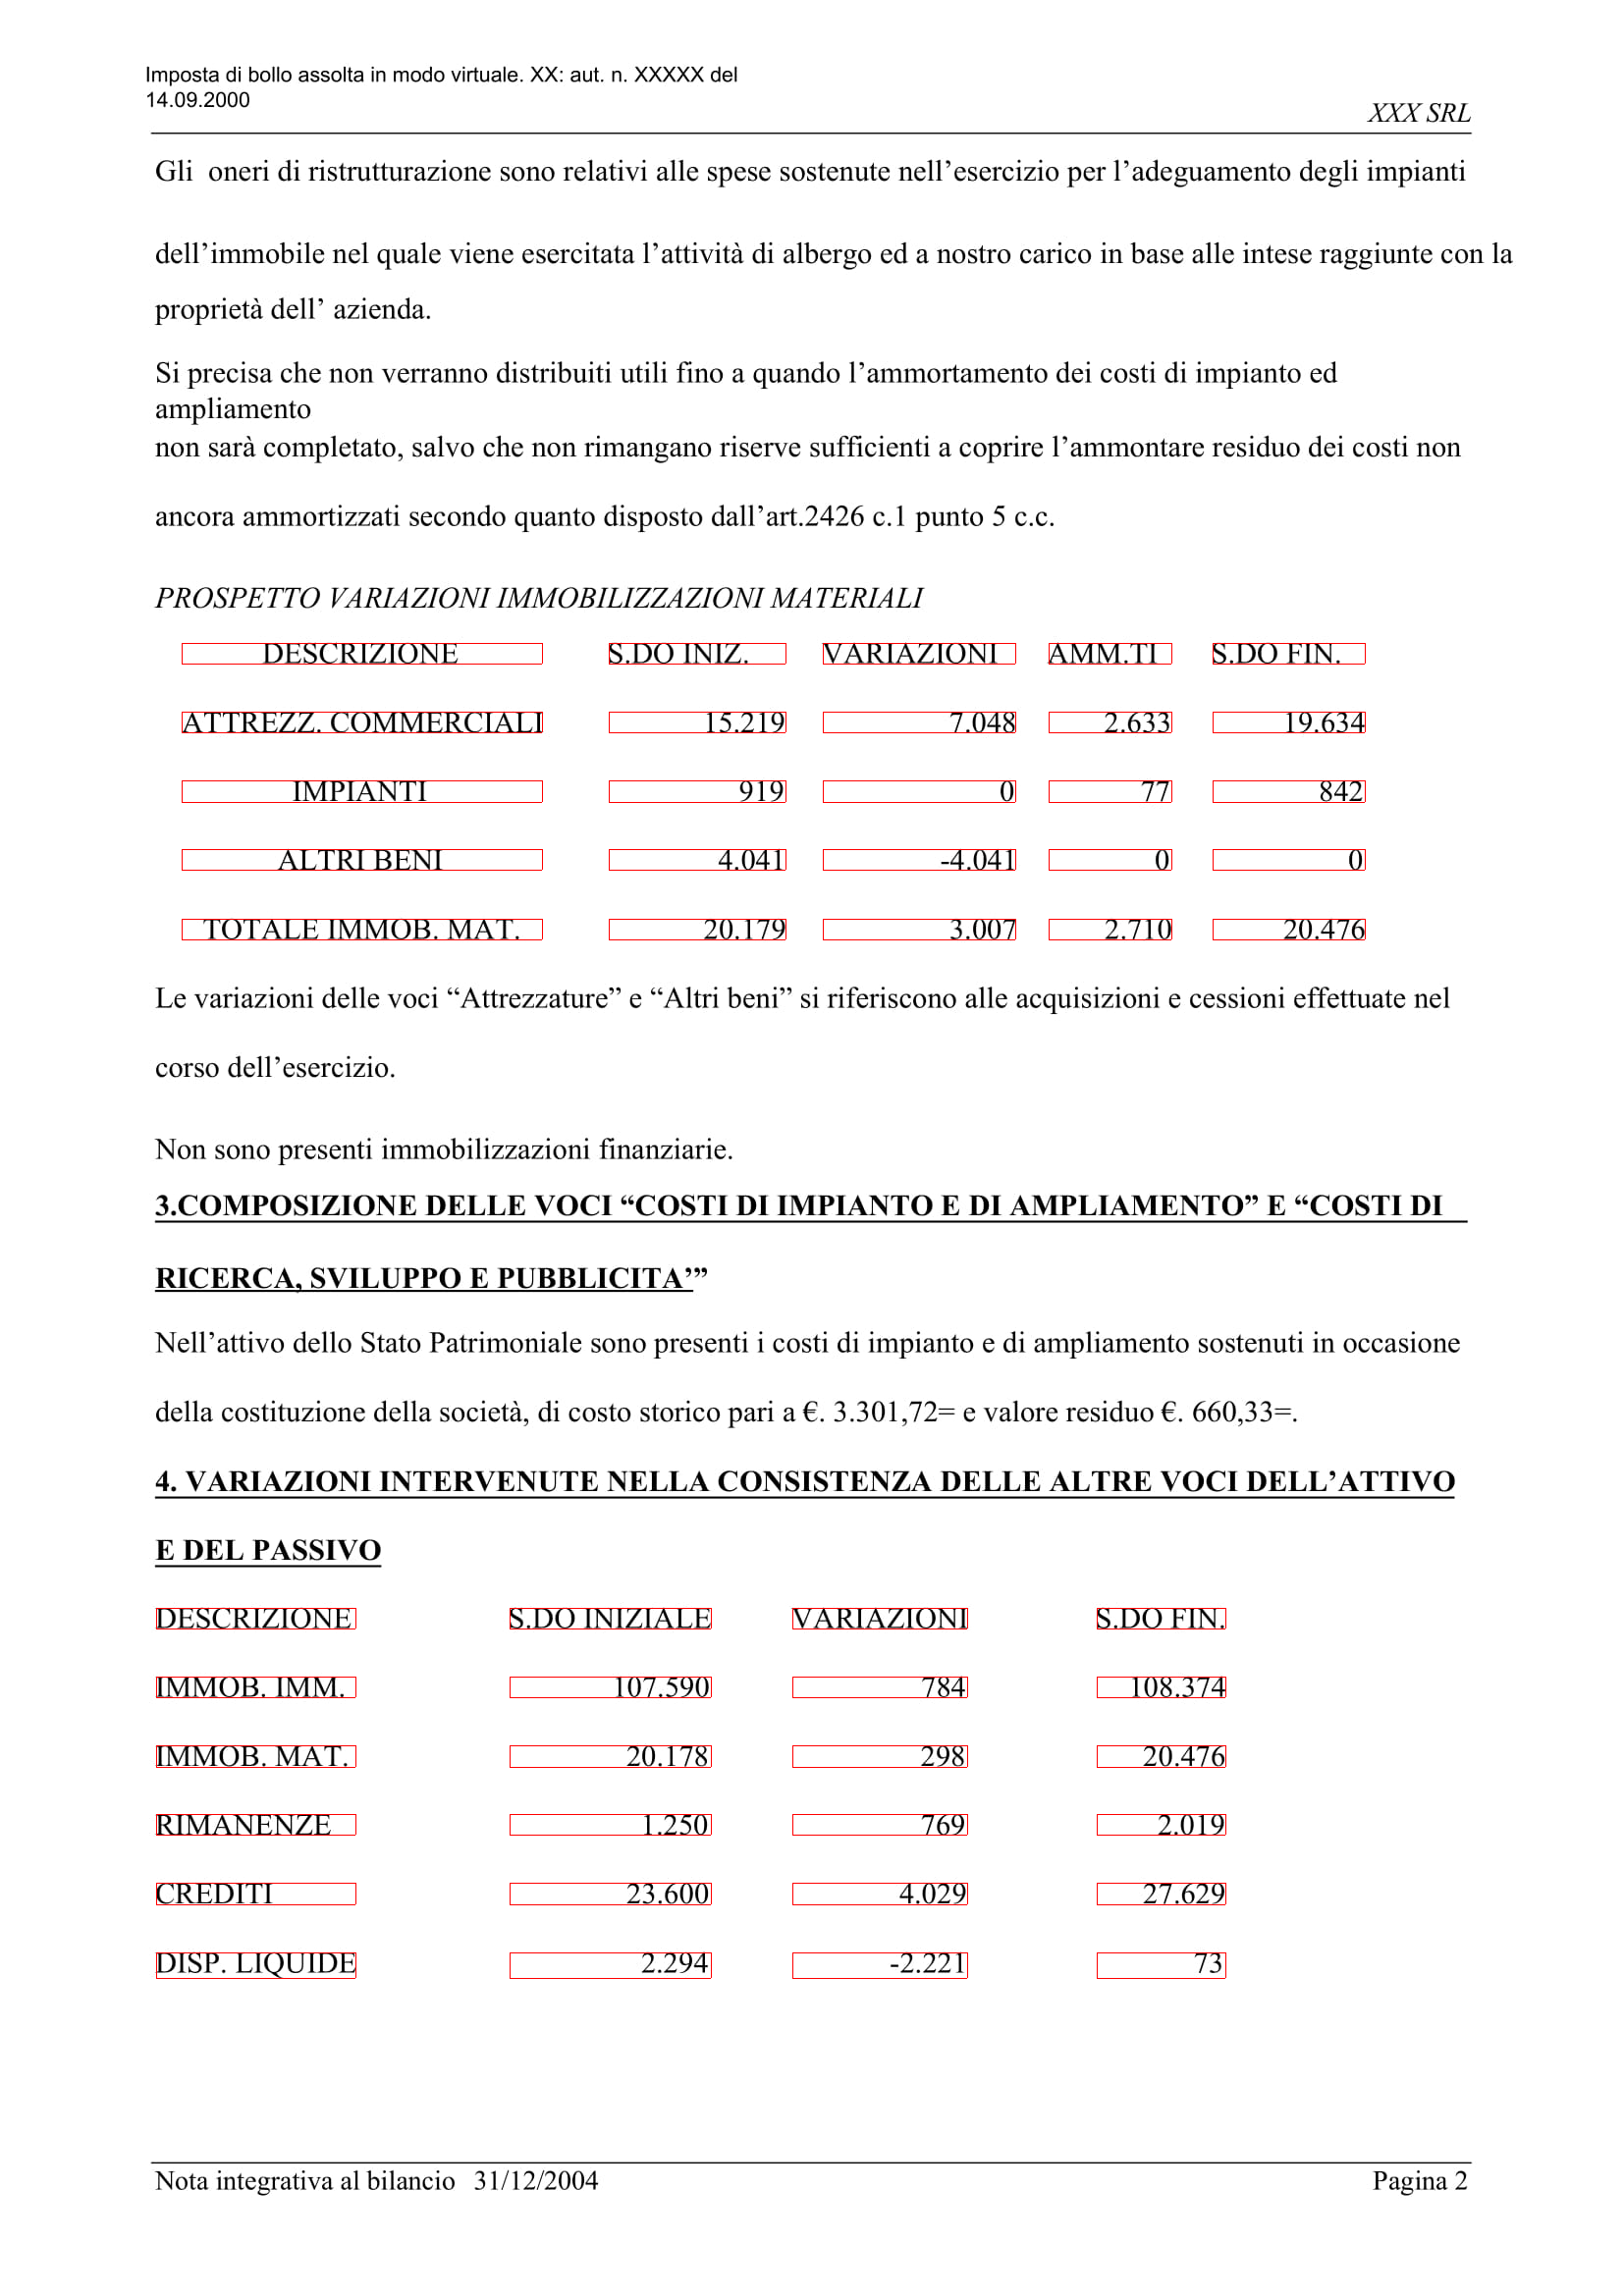
\includegraphics[width=\linewidth]{img/implementation/implem4.png}
\caption{Result of our algorithm: individual bordered cells that represent tables.}
\label{fig:implem4}
\end{subfigure}
\caption{The process of table recognition.}
\label{fig:implemTableRecogniton}
\end{figure}

\chapter{Results}

In this chapter, we analyze the performance of our software and compare its results to those of the Tesseract \emph{table find} algorithm. For these purposes, we use our own testing set of 155 images containing one or more tables. We deliberately chose images that were not scanned or disrupted in any way, as this would only further disrupt the results from Tesseract recognition. As both our algorithm and Tesseract rely on the correctness of the recognized characters and our goal is to test the table recognition, we did everything we could to improve the Tesseract recognition process. 

\section{Performance measures}

As already mentioned, Tesseract is a robust engine. Its recognition and its functions therefore take a great amount of time, which is also the reason why the time complexity of our implementation is significantly higher. 

In comparison, when we run our software on a single image ($1654\times2339$ with the size 675 KB), the absolute time of recognition is 11.6 seconds. Tesseract's API initialization uses 9.6 seconds of this time (with its \emph{recognize()} function that performs the character and line recognition in 9.2 seconds), and our functions for saving results (which use the calls of Leptonica) take 0.5 seconds. About 1.4 seconds is consumed by our \emph{init\_textlines()} function, which also uses the calls of the Tesseract API. However, this function needs to iterate over all symbols and textlines multiple times, which also adds to the time complexity. The time complexity of the other functions (which is below 0.1 seconds) is therefore negligible compared to the already stated performance measures.

We ran a performance test on all 155 images to provide a better concept of the amount of time that our software spends on each function. We did not add any preprocessing, as it is a part of the Leptonica library and therefore does not affect the performance of entirely our functions. Furthermore, upon running a few tests on the preprocessor functions, they seemed to barely affect the performance.

The results from our test were as follows:

\begin{table}[H]
\centering
\begin{tabular}{ccccc}
\toprule
\textbf{All} & \textbf{Tesseract API} & \textbf{Textline initialization} & \textbf{Result saving} & \textbf{Other}\\
\midrule
100\% & 65.94\% & 30.26\% & 2.9\% & 0.9\% \\
\bottomrule
\end{tabular}
\caption{Time complexity of individual functions} 
\label{table:forward-inverted}
\end{table}

The initialization of textlines, however, is tricky. In most of the cases, its time complexity does not exceed 20\%. However, a few images, usually those containing full-page tables, sometimes spent even more time analyzing textlines than with the actual recognition.

In the following sections, we will discuss the options of reducing this time complexity in favor of the accuracy of results. This includes the discussion about the effects of the quality of an image on the results and time complexity, as well as the amount of text in an image on the time complexity.

\section{Effects of image quality}

The quality of the input image greatly affects Tesseract's recognition system and therefore our recognition system.


\section{Effects of preprocessing}

As mentioned multiple times in the previous chapters, preprocessing is a crucial part of any OCR engine, including Tesseract. In this section, we will show its importance along with a few examples of how the recognition results change when only slight tweaks in an image are made.





\section{Comparison to Tesseract's tablefind}


\chapter*{Conclusion}
\addcontentsline{toc}{chapter}{Conclusion}

In this thesis, we explored and reviewed the existing approaches for optical character recognition, and focused on applying its results to the problem of table recognition.

As a main result of the thesis, we have developed a software package that combines the OCR functionality available in the Tesseract library with several methods of image preprocessing, and a newly developed heuristic-based algorithm that aims to improve the available possibilities of table extraction from scanned documents.

We have compared the results obtained from running this combination on a simple testing data set to the results from the TableFind algorithm of Tesseract. While both implementations required similar computational resources for processing the data, our implementation produced more accurate results for more complicated types of table layouts, especially on tables without available border separators, and in cases where the table layout depends e.g.~on subtle differences in cell formatting. Additionally, we have assessed how the resolution and information content of the input image affects the time complexity and output quality of the algorithms.

Despite the improvements in table recognition capabilities, we have observed that the outcome of the recognition still mainly depends on the quality of the input image, and is mostly improved by correct preprocessing.

In the future, we plan to improve the main deficiencies of the whole pipeline, primarily the mentioned preprocessing and several open problems with table recognition summarized in~\cref{sec:future}. From the observed results, we believe that after applying the preprocessing improvements, the table recognition system will produce results of excellent quality.

%%% Bibliography
%%% Bibliography (literature used as a source)
%%%
%%% We employ bibTeX to construct the bibliography. It processes
%%% citations in the text (e.g., the \cite{...} macro) and looks up
%%% relevant entries in the bibliography.bib file.
%%%
%%% The \bibliographystyle command selects, which style will be used
%%% for references from the text. The argument in curly brackets is
%%% the name of the corresponding style file (*.bst). Both styles
%%% mentioned in this template are included in LaTeX distributions.

%\bibliographystyle{alphanat}    %% Author (year)

% \bibliographystyle{unsrt}     %% [number]

%\renewcommand{\bibname}{Bibliography}
%\nocite{*}

%%% Generate the bibliography. Beware that if you cited no works,
%%% the empty list will be omitted completely.

\printbibliography

%%% If case you prefer to write the bibliography manually (without bibTeX),
%%% you can use the following. Please follow the ISO 690 standard and
%%% citation conventions of your field of research.

% \begin{thebibliography}{99}
%
% \bibitem{lamport94}
%   {\sc Lamport,} Leslie.
%   \emph{\LaTeX: A Document Preparation System}.
%   2nd edition.
%   Massachusetts: Addison Wesley, 1994.
%   ISBN 0-201-52983-1.
%
% \end{thebibliography}



%%% Figures used in the thesis (consider if this is needed)
\listoffigures

%%% Tables used in the thesis (consider if this is needed)
%%% In mathematical theses, it could be better to move the list of tables to the beginning of the thesis.
\listoftables

%%% Abbreviations used in the thesis, if any, including their explanation
%%% In mathematical theses, it could be better to move the list of abbreviations to the beginning of the thesis.
%\chapwithtoc{List of Abbreviations}  -- this belongs to 20th century, abbreviations should be defined on the first use

%%% Attachments to the bachelor thesis, if any. Each attachment must be
%%% referred to at least once from the text of the thesis. Attachments
%%% are numbered.
%%%
%%% The printed version should preferably contain attachments, which can be
%%% read (additional tables and charts, supplementary text, examples of
%%% program output, etc.). The electronic version is more suited for attachments
%%% which will likely be used in an electronic form rather than read (program
%%% source code, data files, interactive charts, etc.). Electronic attachments
%%% should be uploaded to SIS and optionally also included in the thesis on a~CD/DVD.
%%% Allowed file formats are specified in provision of the rector no. 72/2017.
\appendix
\chapter{Software user guide}
\xxx{fill this}
\chapter{Contents of the enclosed CD}
\xxx{fill this}

\openright
\end{document}
